
\documentclass[]{interact}


\usepackage[numbers,sort&compress]{natbib}% Citation support using natbib.sty
\bibpunct[, ]{[}{]}{,}{n}{,}{,}% Citation support using natbib.sty
\renewcommand\bibfont{\fontsize{10}{12}\selectfont}% Bibliography support using natbib.sty
\makeatletter% @ becomes a letter
\def\NAT@def@citea{\def\@citea{\NAT@separator}}% Suppress spaces between citations using natbib.sty
\makeatother% @ becomes a symbol again

\usepackage{booktabs}
\usepackage{tikz}
\usepackage{subcaption}
\usepackage{amsmath,amssymb}
\usepackage{amsthm}
\usepackage{pgfplots}
\usepackage{accents}
\usepackage{units}
\usepackage{array}
\usepackage{mathtools}
\usepackage{hyperref}
\usepackage{floatrow}
\usepackage{algorithm}
\usepackage{algorithmic}

\DeclareMathOperator{\E}{\mathbb{E}}
\DeclareMathOperator{\pr}{\mathbb{P}}
\DeclarePairedDelimiter{\ceil}{\lceil}{\rceil}
\DeclarePairedDelimiter{\floor}{\lfloor}{\rfloor}
\newcommand{\STAB}[1]{\begin{tabular}{@{}c@{}}#1\end{tabular}}
\usepgfplotslibrary{statistics}
\newlength{\dhatheight}
\newcommand{\doublehat}[1]{%
    \settoheight{\dhatheight}{\ensuremath{\hat{#1}}}%
    \addtolength{\dhatheight}{-0.15ex}%
    \hat{\vphantom{\rule{1pt}{\dhatheight}}%
    \smash{\hat{#1}}}}
\DeclareMathOperator*{\argmin}{\arg\!\min}
\DeclareMathOperator*{\argmax}{\arg\!\max}\makeatletter
\makeatother


\theoremstyle{plain}% Theorem-like structures provided by amsthm.sty
\newtheorem{Theorem}{Theorem}[section]
\newtheorem{lemma}[Theorem]{Lemma}
\newtheorem{corollary}[Theorem]{Corollary}
\newtheorem{proposition}[Theorem]{Proposition}

\theoremstyle{definition}
\newtheorem{definition}[Theorem]{Definition}
\newtheorem{example}[Theorem]{Example}

\theoremstyle{remark}
\newtheorem{remark}{Remark}
\newtheorem{notation}{Notation}

\newtheorem{example_game}{Example Game}

\begin{document}
%\articletype{ARTICLE TEMPLATE}% Specify the article type or omit as appropriate
\title{Stratified Finite Empirical Bernstein Sampling}
%\author{
%\name{A.~N. Author\textsuperscript{a}\thanks{CONTACT A.~N. Author. Email: latex.helpdesk@tandf.co.uk} and John Smith\textsuperscript{b}}
%\affil{\textsuperscript{a}Taylor \& Francis, 4 Park Square, Milton Park, Abingdon, UK; \textsuperscript{b}Institut f\"{u}r Informatik, Albert-Ludwigs-Universit\"{a}t, Freiburg, Germany}
%}
\author{
\name{Mark Alexander Burgess\textsuperscript{a}\footnote{ORCID: 0000-0003-1627-9125 and 0000-0002-5055-3004 respectively}\thanks{Corresponding author: Mark Alexander Burgess. Email: mark.burgess@anu.edu.au, alternatively: markburgess1989@gmail.com} and Archie C. Chapman\textsuperscript{b}}
\affil{\textsuperscript{a}Australian National University, College of Engineering and Computer Science, Canberra; \textsuperscript{b}The University of Sydney, School of Electrical and Information Engineering, Sydney}
}

\maketitle

\begin{abstract}
We derive a concentration inequality for the uncertainty in the mean computed by stratified random sampling, and provide an online sampling method based on this inequality.
Our concentration inequality is versatile and considers a range of factors including: the data ranges, weights, sizes of the strata, the number of samples taken, the estimated sample variances, and whether strata are sampled with or without replacement.
Sequentially choosing samples to minimize this inequality leads to a online method for choosing samples from a stratified population.
We evaluate and compare the effectiveness of our method against others for synthetic data sets, and also in approximating the Shapley value of cooperative games.
Results show that our method is competitive with the performance of Neyman sampling with perfect variance information, even without having prior information on strata variances.
We also provide a multidimensional extension of our inequality and discuss future applications.
\end{abstract}

\begin{keywords}
Concentration Inequality;
Empirical Bernstein Bound;
Stratified Random Sampling;
Shapley Value Approximation;
\end{keywords}



\section{Introduction}

Stratified sampling is a statistical method for estimating the mean of a population by partitioning it into mutually exclusive subgroups, or strata, and applying a sampling estimator to each stratum, before weighting and combining these estimates to form an estimate of the population mean.
For example, to poll the population of a country's support for a particular government policy, we can selectively poll the different demographic regions within the country.
For instance, if we know that regions $A$,$B$ and $C$ contain 10\%, 40\% and 50\% of the population, and sampling shows support levels for a policy of 2\%, 70\% and 30\%, respectively, then we can estimate that 43.2\% of the total population supports the policy.

Stratified sampling can lead to improved reliability in estimation under certain conditions, such as: 
when the population is easily divided into strata, in which there is less variance in each stratum than across them all; 
when the size of the strata are known, and; 
when sampling selectively from each strata is possible \cite{1938.10503378,10.2307/23339498}.
If it is possible to sample selectively between the strata, then there is a further question of how to conduct that sampling most efficiently.

In this paper we propose a process of sampling in order to maximally reduce the uncertainty in the population mean estimate, 
and to do this we develop a expression associated with that uncertainty.
The expression takes the form of a \textit{concentration inequality}, specifically, a \textit{stratified empirical Bernstein bound} (SEBB),
developed under the assumption that the data values have bounded support. 
This inequality considers factors such as: 
the sizes of all the strata and the proportion of each that are sampled; 
the sample variances of the samples from each of the strata;
the differences in the range of data of each strata;
any additional importance weightings on the strata, and; 
whether any (or all) of the strata are sampled with or without replacement.

Using this inequality, we then propose an online method for sequentially sampling in order to maximally reduce this bound at each iteration, called the \textit{stratified empirical Bernstein method} (SEBM).
By numerically evaluating the SEBM, we demonstrate its value in sampling and estimation applications.
Moreover, we show that it can assist in computational tasks --- particularly those that involve the calculation of expectation values, as sampling is a straightforward way of approximating them.
Specifically, in this work, we consider the calculation of the \textit{Shapley value}, a solution concept from cooperative game theory, as a computational task to which we can apply our sampling method and demonstration of its utility.
Taken together, these results show that SEBM is competitive with the widely-used Neyman sampling method, that assumes perfect variance information, even when SEBM does not have prior information on strata variances.


The remainder of the paper is as follows.
The next section reviews background material and sets the context of the paper. 
Section~\ref{sec:components} provides several lemmas that are components of our derivation. Building on this, in Section~\ref{sec:constructing} we provide the full derivation of our concentration inequality, SEBB, and online sampling method, SEBM, which are the main technical contributions of the paper. 
For evaluation, Section~\ref{sec:application} examines the effectiveness of SEBM in the context of synthetic data sets, 
while Section~\ref{sec:shapley} evaluates its performance on the task of approximating the Shapley value via sampling estimation.
Section~\ref{sec:discussion} discusses the results of these two sets of numerical evaluations, and analyze the reasons for the effectiveness of our sampling method.
Finally, Section~\ref{sec:multi} gives an extension of SEBB and SEBM to multidimensional data.  
Section~\ref{sec:future} concludes.


\section{Background}\label{sec:background}

Stratified sampling is a well known sampling technique in statistics and research, with many applications, including polling \cite{2015PLoSO..1032850H}, auditing \cite{Stark:2009:RPA:1720420.1720456,Miratrix:2009:EAU:1720420.1720453} and medical trials \cite{f7d2c1e6d03c463383ba9f702c3b4dac,doi:10.1093/biomet/73.1.1,Borgan2000}.
Stratified sampling is often conducted as a two-stage process, 
particularly when it is unclear how to stratify the population, or how large the resulting strata would be.
Under this process, the first stage consists of sampling the population uniformly at random, and collecting the values of readily observable auxiliary variables, in order to estimate the sizes of potential strata by those variables.
In the second stage, the strata are chosen and sampled with respect to the information gathered in the first stage, and the total population estimate is computed \cite{LEGG200955}.

One well-known method of estimating efficient strata sizes is via \textit{inverse probability weighting} methods such as the \textit{Horvitz-Thompson estimator} \cite{10.2307/2280784}. 
However, these estimators are sometimes seen to perform quite badly in practice \cite{saegusa2013,Breslow2015}. 
Moreover, these estimator do not directly address the prior problem of how to optimally break the population into strata based on the values of the auxiliary variables  \cite{2015PLoSO..1032850H,DBLP:journals/jmma/KhanAK09,CIS-196251}.

In other situations, the strata and their sizes are naturally given, 
or the first stage of the two-stage process above may be assumed to have been conducted ideally.
In these situation, there exists a further problem of how to allocate the finite number of second-stage samples between the strata. 
For instance, one could choose to sample equally between strata, proportional to the sizes of the strata, or proportional to the variance of the strata.
The last option is often considered in theory and practice, and is called \textit{Neyman allocation} (sometimes called `optimum' allocation) \cite{1938.10503378,10.2307/23339498}. 
This approach assumes knowledge of the variances of the strata; however, in practice it is often the case that strata variance can only be estimated, either as part of the first stage or as the sampling proceeds \cite{etore2010,DBLP:journals/tsg/OBrienGR15}.

Finally, even once the samples are taken from the various strata, there is still the question of how to compute appropriate confidence bounds on the final estimate.
In the voting verification context, there exist some specialized bounds  \cite{Miratrix:2009:EAU:1720420.1720453,Bentkus2003}, but in the more general case there is some degree of discussion of what bounds should be used \cite{Stark:2009:RPA:1720420.1720456}.
The confidence bounds that are derived critically depend on what assumptions are made about the underlying populations.

In particular, \textit{Hoeffding's inequality} \cite{hoeffding1} is used as a bound under the assumption that the underlying population has bounded data support, or are drawn from a finite interval \cite{Bentkus2003,Stark:2009:RPA:1720420.1720456}.
Hoeffding's inequality can be used to produce a very conservative confidence interval that is sensitive only to the width of the data value bounds and the number of samples taken, and it is also most directly suitable for sampling with replacement. 
In contrast, other concentration inequalities, such as \textit{Chebychev's inequality}, 
are sensitive to the sample variance but not the width of the data.

Recently, Maurer and Pontil \cite{Maurer50empiricalbernstein} developed a bound, which they named as an \textit{empirical Bernstein bound} (EBB), as a concentration of measure for the sample mean of a single (unstratified) population
(some similar bounds being published about that time, \cite{zbMATH05552995,10.1007/978-3-540-75225-7_15}). 
EBBs are is sensitive to the data width and sample variance.
They have replaced Hoeffding's inequality in a number of computational applications \citep{Zia-UrRehman2012,Mnih:2008:EBS:1390156.1390241,DBLP:conf/aaai/ThomasTG15,Carpentier:2011:UAA:2050345.2050366}.
The derivation of Maurer and Pontil's EBB extendeds from entropic \cite{Maurer_concentrationinequalities} and Chernoff concentration inequalities, which are combined using union bounds.

Beyond this, sampling \textit{without replacement} offers the opportunity to further tighten the bounds over the sampling-with-replacement case. 
For example, the refinement that is possible was first demonstrated by Serfling \cite{serfling1974} with a martingale argument.
More recently, Bardenet and Maillard \cite{bardenet2015} improved on Serfling's result with a reverse martingale argument, and created an EBB suitable to the case of sampling without replacement.

Our key observation is that the components of these analyses can be combined together to create a closed form analytical concentration inequality tailored for stratified random sampling, which is a primary subject of this paper.


\section{Preliminaries}\label{sec:components}

We now state nine lemmas across the next three sections, which we use later to derive our stratified empirical Bernstein bound (SEBB) and method (SEBM). 
Specifically, in Section~\ref{subsec:fundamentals}, we provide three lemmas, which show how probability bounds are related to the moment generating function, how probability bounds can be combined, and a useful algebraic relationship regarding the sample variance.
Then, in Section~\ref{subsec:mgf}, we provide three bounds on the moment generating functions of random variables.
Last, in Section~\ref{sec:without_replacement}, we derive three lemmas that relate the moment generating function to the sample means of random variables with and without replacement.


\subsection{Fundamental results}\label{subsec:fundamentals}

The first lemma is an often-used and rather weak result used to fuse simple statements of probability:

\begin{lemma}[Probability Union]\label{prob_union}
For any random variables $a,b,c$:\\
$~~\pr(a>c) \; \le \; \pr(a>b) + \pr(b>c)$
\end{lemma}
%\begin{proof}
%For any events $A$ and $B$, $\p(A\cup B) \; \le \; \p(A)+\p(B)$ hence:
%\[\p\left((a>b) \cup (b>c)\right) \;\le\; \p(a>b) + \p(b>c).\]
%If $a>c$, then $(a>b) \cup (b>c)$ is true irrespective of $b$, so:
%\[\p(a>c) \;\le\; \p\left((a>b) \cup (b>c)\right).\qedhere\]
%\end{proof}
\noindent
This relationship is a well known and useful tool for settings where the probability relationship between $a$ and $c$ is unknown but the relationship between $a$ and some $b$, and also between that $b$ and $c$ is known.

The next lemma is a straightforward result of algebra that relates the sample squares about the mean to the sample variance.
\begin{lemma}[Variance Relation]\label{variance1}
Let $X$ be a random variable with mean $\mu$. 
For $n$ samples of $X$, $\{x_k\}_{k=1,\ldots,n}$, 
the sample mean, $\hat{\mu}=\frac{1}{n}\sum_k x_k$, 
biased sample variance, $\hat{\sigma}^2=\frac{1}{n}\sum_k (x_k-\hat{\mu})^2$, 
and average of sample squares about the mean, $\hat{\sigma}_0^2 = \frac{1}{n}\sum_k (x_k-\mu)^2$, 
are related such that:
\[
\textstyle\hat{\sigma}_0^2-\hat{\sigma}^2 = \left(\hat{\mu}-\mu\right)^2.
\nonumber
\]
\end{lemma}
%\begin{proof} 
%By definition:
%\[\textstyle\hat{\sigma}^2 =\frac{1}{n}\sum_i\left(x_i-\frac{1}{n}\sum_jx_j \right)^2 =\frac{1}{n}\sum_ix_i^2-\frac{1}{n^2}\sum_i\sum_jx_ix_j\]
%and: 
%\[\hat{\sigma}_0^2 =\frac{1}{n}\sum_i\left(x_i-\mu \right)^2 =\frac{1}{n}\sum_ix_i^2 - \frac{2\mu}{n}\sum_ix_i + \mu^2\]
%therefore: 
%\[\textstyle\hat{\sigma}_0^2-\hat{\sigma}^2 =\frac{1}{n^2}\sum_i\sum_jx_ix_j - \frac{2\mu}{n}\sum_ix_i + \mu^2 = \left(\frac{1}{n}\sum_jx_j-\mu\right)^2\qedhere\]
%\end{proof}
\noindent
This result is used later to create bounds for the sample variance from bounds on the sample squares about the mean.
In order to create such probability bounds, we make repeated use of the next, which extends directly from Markov's inequality and encompasses a range of inequalities called \textit{Chernoff bounds}:

\begin{lemma}[Chernoff Bound]\label{chernoff1}
For a random variable $X$, and for any $s>0$ and $t$:
\[
\textstyle\pr(X\ge t)\le\E\left[\exp(sX)\right]\exp(-st) 
\nonumber
\]
\end{lemma}
%\begin{proof}
%$\textstyle\p(X\ge t) =  \p\left(\exp(sX)\ge \exp(st)\right) \le \E\left[\exp(sX)\right]\exp(-st)$\\by Markov's inequality.
%\end{proof}
\noindent
Many well-known inequalities follow from upper bounds for $\E\left[\exp(sX)\right]$, also known as the \textit{moment generating function}.

\subsection{Bounds on the Moment Generating Function}\label{subsec:mgf}

The next three lemmas give three of these upper bounds for moment generating functions, from which we create our probability inequalities of interest.
The first is well known and sometimes called \textit{Hoeffding's Lemma} \citep{hoeffding1} and is stated here without proof:

\begin{lemma}[Hoeffding's Lemma]\label{expectation0}
For a random variable $X$ that is of finite support on the interval $a\le X\le b$, with width $D=b-a$, and for any $s>0$:
\[
\E\left[\exp(s(X-\E[x]))\right] \le\exp\left(\frac{1}{8}D^2s^2\right).
\nonumber
\]
\end{lemma}
\noindent
The second lemma is very much like Hoeffding's Lemma, except it involves information about the variance of the random variable.
The proof of this result is included because it is useful in explaining our own approach.

\begin{lemma}\label{expectation1}
For a random variable $X$ that is bounded on an interval $a\le X\le b$ with $D=b-a$ and variance $\sigma^2$, and any $s>0$:
\[
\E\left[\exp(s(X-\E[x]))\right] 
\le\exp\left(\left(\frac{D^2}{17}+\frac{\sigma^2}{2}\right)s^2\right)
\nonumber
\]
\end{lemma}
\begin{proof}

We assume without loss of generality that $X$ is centered to have a mean of zero.
Then we construct an upper bound for $\E\left[\exp(sX)\right]$ in terms of $D$ by a parabola over $\exp(sX)$ for the permitted values of $X$.

There exists an $\alpha,\beta,\gamma$ (see Appendix\ref{appendix1}) such that $\alpha s^2X^2+\beta sX+\gamma\ge \exp(sX)$, and for all $a\le X\le b$:
\[
E\left[\exp(sX)\right] \le \E[\alpha s^2X^2+\beta sX+\gamma] = \alpha s^2\E[X^2]+\gamma = \alpha s^2\sigma^2+\gamma
\nonumber\]
Where it follows that:
\begin{equation}\label{eqn:intermediate_lemma3.5}
E\left[\exp(sX)\right] \le\left(\frac{\sigma^2}{b^2}\exp\left(s\left(b+\frac{\sigma^2}{b}\right)\right) + 1\right)\exp\left(-\frac{s\sigma^2}{b}\right)\left(\frac{\sigma^2}{b^2} + 1\right)^{-1}.
\nonumber 
\end{equation}
The expression in \eqref{eqn:intermediate_lemma3.5} is monotonically increasing with $b$, and $D>b$, therefore:
\begin{equation}\label{eq:part1}
\log(E\left[\exp(sX)\right]) \le \log\left(\frac{\sigma^2}{D^2}\exp\left(s\left(D+\frac{\sigma^2}{D}\right)\right) + 1\right)-\frac{s\sigma^2}{D} - \log\left(\frac{\sigma^2}{D^2} + 1\right)
\end{equation}
Given that for any $\kappa,x\ge 0$, that: 
\begin{equation}\label{eq:part2}
\log(\kappa\exp(x)+1)\le\log(\kappa+1)+\frac{x\kappa}{\kappa+1}+x^2\frac{\frac{1}{17}+\frac{\kappa}{2}}{(\kappa+1)^2}
\end{equation}
Thus letting $\kappa=\frac{\sigma^2}{D^2}$ and $x=s(D+\sigma^2/D)$ if follows that:
\begin{equation}\label{eq:part3}
\log(E\left[\exp(sX)\right]) \le \left(\frac{D^2}{17}+\frac{\sigma^2}{2}\right)s^2\qedhere
\end{equation}
\end{proof}

We note that this process of fitting a parabola over the exponential function bears a strong conceptual relationship with a famous bound developed by Hoeffding \cite{hoeffding1} and Bennett \cite{10.2307/2282438}.

The third bound that we present, on the moment generating function, is similar again, however this time we consider the random variable $X^2$ instead of $X$. 

\begin{lemma}\label{expectation2}
Let $X$ be a random variable of finite support on an interval $a\le X\le b$, with $D=b-a$ and variance $\sigma^2 = \E[(X-\E[x])^2] = \E[X^2]-\E[X]^2$. Then for any $q>0$:
$$\E[\exp(q(\sigma^2-(X-\E[X])^2))] \le \exp\left(\frac{1}{2}\sigma^2q^2D^2\right)$$
\end{lemma}
\begin{proof}
We assume without loss of generality (and for ease of presentation) that X is centered to have a mean of zero.
We construct an upper bound for $\E\left[\exp(-qX^2)\right]$ in terms of $D$ by a parabola over $\exp(-qX^2)$ for the permitted values of $X$.

For an $\alpha,\gamma$ such that $\alpha X^2+\gamma\ge \exp(-qX^2)$ then:
$$ \E[\exp(-qX^2)] \le \alpha \sigma^2 + \gamma.$$
If $d=\max(b,-a)$ we can choose $\gamma=1$ and $\alpha=(\exp(-q d^2)-1)d^{-2}$ (see figure \ref{fig:graph111}), Thus:
\begin{align*}
\E[\exp(-q X^2)] &\le \frac{\sigma^2}{d^2}\exp(-q d^2)-\frac{\sigma^2}{d^2} + 1\le \frac{\sigma^2}{D^2}\exp(-q D^2)-\frac{\sigma^2}{D^2} + 1 \\
&\le \exp\left(\log\left(\frac{\sigma^2}{D^2}\exp(-q D^2)-\frac{\sigma^2}{D^2} + 1\right)\right)
\end{align*}
Given that for any $0\le \kappa \le 0.5$ and $x\le 0$ that: $$\log\left(\kappa\exp(x)-\kappa + 1\right) \le \kappa x+\frac{1}{2}\kappa(1-\kappa)x^2$$
Letting $\kappa=\frac{\sigma^2}{D^2}$ and $x=-qD^2$, which is valid by Popoviciu's inequality \cite{zbMATH05780164} $\sigma^2\le D^2/4$, then:
$$ \E[\exp(-q X^2)] \le \exp\left(\frac{1}{2}\sigma^2q^2(D^2-\sigma^2)-\sigma^2q\right) \le \exp\left(\frac{1}{2}\sigma^2q^2D^2-\sigma^2q\right)$$
and the result follows by multiplying by $\exp(q\sigma^2)$.
\end{proof}

The three inequalities above, Lemmas \ref{expectation0},\ref{expectation1} and \ref{expectation2}, are used in the derivation of our stratified sampling concentration inequality in Section~\ref{sec:constructing}.

\subsection{The Moment Generating Function of Sample Means}\label{sec:without_replacement}

In order to use the previous bonds on the moment generating function we need an inequality relating the moment generating function of a random variable, with the moment generating function of the average of samples of that random variable.
To do this we state three further inequalities, where the first one (Lemma~\ref{martingale1}) is most appropriate for sampling with replacement, and the second and third (Lemma~\ref{hoeffdings_reduction} and Lemma~\ref{martingale0}) can optionally be used in the context of sampling without replacement.

\begin{lemma}[Replacement Bound]\label{martingale1}
Let $X$ be a random variable that is bounded $a\le X\le b$ with a mean of zero, with $D=b-a$ and variance $\sigma^2$.
Let $\chi_m = \frac{1}{m}\sum_{i=1}^mX_i$ be the average of $m$ independently drawn (with replacement) samples of this random variable.
If there exists an $\alpha, \beta \ge 0$ such that for any $s>0$ that $\E[\exp(sX)]\le\exp((\alpha D^2 +\beta \sigma^2) s^2)$ then:
$$\textstyle\E[\exp(s\chi_m)]\le\exp(\alpha s^2D^2\frac{1}{m} +\beta s^2\sigma^2 \frac{1}{m}) = \exp((\alpha D^2{\Omega}_m^n +\beta\sigma^2 {\Psi}_m^n)s^2)$$
where ${\Omega}_m^n = {\Psi}_m^n = \frac{1}{m}$
\end{lemma}
\begin{proof} 
By the independence of samples, we have:
\[\E[\exp(s\chi_m)]=\E\left[\exp\left(\frac{s}{m}\sum_{i=1}^mX_i\right)\right]=\prod_{i=1}^m\E\left[\exp\left(\frac{s}{m}X\right)\right]\] 
Thus:
\[\E[\exp(s\chi_m)] \le \exp\left(\frac{s^2}{m^2}\sum_{i=1}^m\left(\alpha D^2 +\beta \sigma^2\right) \right) \qedhere\]
\end{proof}

%The requirement that the mean of the random variable is zero is useful as further derivations are applied to random variables which are shifted such as to have a mean of zero ie. $X-\E[X]$.
These inequalities are sufficient for all the further derivations that we conduct. 
However, for the case of sampling without replacement, 
there is an alternative result that can be directly substituted, given in Lemma~\ref{martingale0}, below, which can be tighter in certain cases. 
We give its form and derivation, which is included for completeness but is not part of the main results presented in the paper.
Before this, particular note must be made that the inequality above, Lemma~\ref{martingale1} can be used in the context of either sampling with or without replacement.
In contrast, Lemma~\ref{martingale0} can only be used when sampling without replacement. 
This distinction was shown to be true by Hoeffding \cite{hoeffding1}, 
and is stated here without proof:

\begin{lemma}[Hoeffding's reduction]\label{hoeffdings_reduction}
let $X=(x_1,\dots,x_n)$ be a finite population of $n$ real points, let $X_1,\dots,X_n$ denote a random sample without replacement from $X$ and $Y_1,\dots,Y_n$ denote a random sample with replacement from $X$. 
If $f:\mathbb{R}\rightarrow\mathbb{R}$ is continuous and convex, then:
$$\textstyle \E\left[f\left(\sum_{i=1}^mX_i\right)\right]\le\E\left[f\left(\sum_{i=1}^mY_i\right)\right] $$
\end{lemma}

we now state an inequality regarding the moment generating function of the average of samples taken specifically \textit{without replacement}.

When the sampling takes place without replacement the inequality of Lemma~\ref{martingale1} can potentially be improved to take advantage of the finite size of the population.
This inequality extends an important martingale inequality from \cite{bardenet2015}:

\begin{lemma}[Martingale Bound]\label{martingale0}
For finite data $x_1,x_2,\dots x_n$ that is bounded $a\le x_i\le b$, and has a mean of zero and variance $\sigma^2=\frac{1}{n}\sum_{i=1}^nx_i^2$, denote $X_1,X_2,\dots,X_n$ the random variables corresponding to the data sequentially drawn randomly without replacement, and $\chi_m$ the average of the first $m$ of them.
If for any random variable $Z$ with a mean of zero such that $a\le Z\le b$ and $D=b-a$, with variance $\sigma_Z^2$ that there exists an $\alpha, \beta \ge 0$ such that for any $s>0$ that $\E[\exp(sZ)]\le\exp((\alpha D^2 +\beta \sigma_Z^2) s^2)$ then:
\begin{align*}\E[\exp(s\chi_m)]&\le\exp\left(\alpha s^2D^2\sum_{k=m}^{n-1}\frac{1}{k^2} +\beta s^2\sigma^2 \sum_{k=m}^{n-1}\frac{n}{k^2(k+1)}\right)\\ &\le \exp((\alpha D^2\bar{\Omega}_m^n +\beta\sigma^2 \bar{\Psi}_m^n)s^2)\end{align*}
where $\bar{\Omega}_m^n = \sum_{k=m}^{n-1}\frac{1}{k^2}\approx \frac{(m+1)(1-m/n)}{m^2}$ and $\bar{\Psi}_m^n = \sum_{k=m}^{n-1}\frac{n}{k^2(k+1)}\approx \frac{n+1-m}{m^2}$.
\end{lemma}
\begin{proof}
Observe that:
\begin{align*}
\chi_m 
& =\frac{1}{m}\sum_{i=1}^{m}X_i = \chi_{m+1}+\frac{1}{m}(\chi_{m+1}-X_{m+1})\\
& =(\chi_m-\chi_{m+1})+(\chi_{m+1}-\chi_{m+2}) + \dots + (\chi_{n-1}-\chi_n)\\
& =\frac{1}{m}(\chi_{m+1}-X_{m+1})+\frac{1}{m+1}(\chi_{m+2}-X_{m+2}) + \dots + \frac{1}{n-1}(\chi_n-X_n).
\end{align*} 
Then because:
$$\exp(s\chi_m)=\prod_{k=m}^{n-1}\exp\left(\frac{s}{k}(\chi_{k+1}-X_{k+1})\right),$$
we also have that: 
$$\E[\exp(s\chi_m)]=\E\left[\prod_{k=m}^{n-1}\E\left[\exp\left(\frac{s}{k}(\chi_{k+1}-X_{k+1})\right)|\chi_{k+1}\dots \chi_n\right]\right]$$
by repeated application of the Law of total expectation. 
Since:
$$\E[X_{k+1}|\chi_{k+1}\dots \chi_n]=\chi_{k+1},$$ 
then $\chi_{k+1}-X_{k+1}$ is a random variable with a mean of zero bounded within width $D$, and it also has a variance given by: 
\begin{equation}\label{approx1} 
\sigma_{k+1}^2 = \frac{n\sigma^2-\sum_{j=k+1}^nX_j^2}{n-(n-k-1)} - \chi_k^2 \le \frac{n\sigma^2}{k+1}
\end{equation}
by application of Lemma~\ref{variance1}. 
Therefore: 
\[\E[\exp(s\chi_m)]\le\exp\left(\sum_{k=m}^{n-1}\left(\alpha D^2 +\beta \frac{n\sigma^2}{k+1}\right) \frac{s^2}{k^2}\right)\qedhere\]
\end{proof}


This martingale result relates the moment generating function bound of the average of finite variables relative to their mean, 
to the moment generating function bounds of the  differences of the incremental averages relative to their mean. 
We note that this result could be made much stronger by working around the use of Equation~\eqref{approx1}, 
but this comes at a cost of increased mathematical complexity.

Since Lemmas~\ref{martingale0} and~\ref{martingale1} share a common form, and because of Hoeffding's reduction (Lemma~\ref{hoeffdings_reduction}), 
all the derivations that follow that invoke Lemma~\ref{martingale1} have direct analogues using Lemma~\ref{martingale0} for the context of sampling without replacement.
Note, however, that the bound without replacement (Lemma~\ref{martingale0}) may or may not be tighter than the bound with replacement (Lemma~\ref{martingale1}). However, the process of substituting one for the other can be done judiciously on a case-by-case basis to create the tightest possible bound.
All the numerical results in this paper (relevant to sampling without replacement) have been produced with this judicious choice conducted.

\section{The Stratified Finite Empirical Bernstein Bound and Sampling Method}
\label{sec:constructing}

This section contains our main results: 
we derive a novel probability bound for the error of the stratified random sampling estimate, 
and use it to define a sequential stratified sampling algorithm. 
Before this, we begin by precisely defining the context of our derivations, to which our bound applies.

\begin{definition}[Problem context]\label{def:ProblemContext}
Let a population consist of $n$ number of strata of finite data points, 
where $n_i$ is the number of data points in the $i$th stratum.
All values in a stratum are bound within a finite support of width $D_i$.
Denote the mean and variance of the $i$th stratum $\mu_i$ and  $\sigma_i^2$, respectively.
%
In this context, denote values randomly and sequentially drawn (with or without) replacement by $X_{i,1},X_{i,2},\dots,X_{i,n_i}$. 
Then, for the  first $m_i$ of these sample: 
(i) $\chi_{i,m_i}= \frac{1}{m_i}\sum_{j=1}^{m_i}X_{i,j}$ is their average;
(ii)~their biased sample variance is
$\hat{\sigma}_i^2=\frac{1}{m_i}\sum_j^{m_i}(X_{i,j}-\chi_{i,m_i})^2$, and;
(iii)~their unbiased sample variance is $\doublehat{\sigma}_i^2 = m_i\hat{\sigma}_i^2/(m_i-1)$.
We are interested in the average of the means of the strata as weighted by constant positive factors $\{\tau_i \}_{i\in \{1,\dots,n\}}$. 
Throughout our derivation, we temporarily use arbitrary positive variables %intermediary weights
$\{\theta_i \}_{i\in \{1,\dots,n\}}$.
\end{definition}


Given this context, the following two sections contain the derivation of the stratified empirical Bernstein bound (SEBB) 
and the sequential sampling method (SEBM), respectively. 



\subsection{Bound derivation}
The bound is now developed in four theorems, 
which build on each other in sequence:
\begin{enumerate}
    \item Theorem~\ref{thm:1} develops a concentration inequality for the error in the stratified population mean estimate $\sum_{i=1}^n\tau_i\chi_{i,m_i}$ in the context of variance information.
    \item Theorem~\ref{thm:2} is a concentration inequality of the difference between the stratum variances and sample variances in the context the sum of squared stratum mean errors.
    \item Theorem~\ref{thm:3} is an inequality directly about the sum of sample squared stratum mean errors.
    \item Theorem~\ref{thm:SEBM_bound} combines the three previous theorems together using union bounds to create a concentration inequality for the error in the stratified population mean estimate given the sample variances.
\end{enumerate}

We begin with an expression for a probability bound on the absolute error of the weighted stratified sample means about the weighted strata means, which we call a variance-assisted SEBB (stratified empirical Bernstein bound).

\begin{Theorem}[Variance-assisted SEBB]\label{thm:1}
Assuming the context given in Definition~\ref{def:ProblemContext}, and let $\Omega_{m_i}^{n_i}$ and $\Psi_{m_i}^{n_i}$ be given as in Lemma~\ref{martingale1}, then:
\begin{equation}\label{eq1} \pr\left(\left|\sum_{i=1}^n\tau_i(\chi_{i,m_i}-\mu_i)\right|\ge \sqrt{4\log(2/t)\sum_{i=1}^n\left(\frac{1}{17}D_i^2\Omega_{m_i}^{n_i}+\frac{1}{2}\sigma_i^2\Psi_{m_i}^{n_i}\right)\tau_i^2}\right)\le t \end{equation}
\end{Theorem}
\begin{proof}
Applying Lemma~\ref{chernoff1}:
\begin{align*} \pr\left(\sum_{i=1}^n\tau_i\chi_{i,m_i}-\sum_{i=1}^n\tau_i\mu_i\ge t\right)
&\le\E\left[\exp\left(\sum_{i=1}^n\tau_is\left(\chi_{i,m_i}-\mu_i\right)\right)\right]\exp(-st)\\
&= \prod_{i=1}^n\E\left[\exp\left(\tau_is\left(\chi_{i,m_i}-\mu_i\right)\right)\right]\exp(-st) 
\end{align*}
by independence of the sampling between the strata. 
This form is sufficient for Lemma~\ref{martingale1} with Lemma~\ref{expectation1} to apply, resulting in a double-sided tail bound:
$$ \pr\left(\left|\sum_{i=1}^n\tau_i(\chi_{i,m_i}-\mu_i)\right|\ge t\right)\le 2\exp\left(\sum_{i=1}^n\left(\frac{1}{17}D_i^2\Omega_{m_i}^{n_i}+\frac{1}{2}\sigma_i^2\Psi_{m_i}^{n_i}\right)\tau_i^2s^2 - st\right) $$
Minimizing with respect to $s$ and rearranging gives result.
\end{proof}

In most cases, the weights $\tau_i$ can be considered as the probability weights $\tau_i=n_i/(\sum_{j=1}^nn_j)$, 
and in this context this probability bound can be used as-is for a measure of uncertainty in stratified random sampling if the true variances (or alternatively, upper bounds on the true variances) of the strata are known. 
However, in other contexts, the weighted sum of variances must be estimated from the data collected, and to include this factor we develop and incorporate a probability bound for the estimate of the sum of variances (as weighted by arbitrary $\theta_i$), as follows. 


\begin{Theorem}\label{thm:2}
Assuming the context given in Definition~\ref{def:ProblemContext}.
Then with $\Psi_{m_i}^{n_i}$ per Lemma~\ref{martingale1}:
\begin{equation}\label{eq2} \pr\left(\sum_{i=1}^n\theta_i(\sigma_i^2-\hat{\sigma}_i^2 - (\mu_i - \chi_{i,m_i})^2)\ge \sqrt{2\log(1/y)\sum_{i=1}^n\sigma_i^2\theta_i^2D_i^2\Psi_{m_i}^{n_i}}\right) \le y \end{equation}
\end{Theorem}


\begin{proof}
To create a probability bound for the sum of variances (weighted by arbitrary positive $\theta_i$), we consider the average square of samples about the strata means. 
Applying Lemma~\ref{chernoff1} gives:
\begin{align*} 
\pr&\left(\sum_{i=1}^n\theta_i(\sigma_i^2-\frac{1}{m_i}\sum_{j=1}^{m_i}(X_{i,j}-\mu_i)^2)\ge y\right) \\
&\le \E\left[\exp\left(\sum_{i=1}^ns\theta_i\left(\sigma^2-\frac{1}{m_i}\sum_{j=1}^{m_i}(X_{i,j}-\mu_i)^2\right)\right)\right]\exp(-sy)\\
& = \exp(-sy)\prod_{i=1}^n\E\left[\exp\left(\frac{s\theta_i}{m_i}\sum_{j=1}^{m_i}(\sigma^2-(X_{i,j}-\mu_i)^2)\right)\right] 
\end{align*}
by independence of the sampling between the strata. 
This is sufficient for Lemma~\ref{martingale1} with Lemma~\ref{expectation2} to apply, giving:
$$ \pr\left(\sum_{i=1}^n\theta_i(\sigma_i^2-\frac{1}{m_i}\sum_{j=1}^{m_i}(X_{i,j}-\mu_i)^2)\ge y\right) \le \exp\left(\frac{1}{2}\sum_{i=1}^n\sigma_i^2\theta_i^2s^2D_i^2\Psi_{m_i}^{n_i}-sy\right)$$
Minimizing with respect to $s$, rearranging, and applying Lemma`\ref{variance1} gives result.
\end{proof}

This inequality gives the probability bound between the weighted variances of the strata, 
the weighted (biased) sample variances 
and the weighted square error of the sample means.
Although the weighted square error of the sample means may go to zero quickly as additional samples are taken, we nonetheless develop another probability bound to incorporate specific consideration of it.

\begin{Theorem}\label{thm:3}
Assuming the context given in Definition~\ref{def:ProblemContext}.
Then with $\Omega_{m_i}^{n_i}$ as in Lemma~\ref{martingale1}:
\begin{equation}\label{eq1.5} \pr\left(\sum_{i=1}^n\theta_i(\mu_i - \chi_{i,m_i})^2 \ge \frac{\log(2n/r)}{2}\sum_{i=1}^n\theta_iD_i^2\Omega_{m_i}^{n_i}\right) \le r \end{equation}
\end{Theorem}
\begin{proof}
We consider the weighted square error of the sample means:
$$ \pr\left(\sum_{i=1}^n\theta_i(\mu_i - \chi_{i,m_i})^2 \ge r\right) \le 1-\prod_{i=1}^n\pr\left(\theta_i(\mu_i - \chi_{i,m_i})^2 \le r_i\right) $$
$$= 1-\prod_{i=1}^n\left(1-\pr\left(\mu_i - \chi_{i,m_i} \ge \sqrt{\frac{r_i}{\theta_i}}\right) - \pr\left( \chi_{i,m_i}-\mu_i \ge \sqrt{\frac{r_i}{\theta_i}}\right)\right),$$
such that $\sum r_i=r$, by independence of the sampling and probability complementarities.
This is sufficient for us to apply Lemma~\ref{chernoff1} together with Lemmas~\ref{martingale1} and~\ref{expectation0}, giving:
$$ 
\pr\left(\sum_{i=1}^n\theta_i(\mu_i - \chi_{i,m_i})^2 \ge r\right) \le 1-\prod_{i=1}^n\left(1-2\exp\left(-\frac{2r_i}{\theta_iD_i^2\Omega_{m_i}^{n_i}}\right)\right)
$$
Next, choosing $r_i$ to minimize this expression gives:
$$
r_i = \frac{r\theta_iD_i^2\Omega_{m_i}^{n_i}}{\sum_j \theta_jD_j^2\Omega_{m_j}^{n_j}}
$$
Thus:
$$ 
\pr\left(\sum_{i=1}^n\theta_i(\mu_i - \chi_{i,m_i})^2 \ge r\right) \le 1-\prod_{i=1}^n\left(1-2\exp\left( \frac{-2r}{\sum_j\theta_j D_j^2\Omega_{m_j}^{n_j}}\right)\right)
$$
Using $\log(1-(1-\exp(x))^n)\le x+\log(n)$ for negative $x$, and rearranging, gives result.
\end{proof}

This theorem bounds the weighted square error of the sample means.
In the next, and final, step we combine the inequalities of Equations~\eqref{eq1}, \eqref{eq2} and~\eqref{eq1.5} together, to complete our derivation of the SEBB.


\begin{Theorem}[Stratified Empirical Bernstein Bound (SEBB)]\label{thm:SEBM_bound}
Assuming the context given in Definition~\ref{def:ProblemContext}.
Then with $\Omega_{m_i}^{n_i},\Psi_{m_i}^{n_i}$ per Lemma~\ref{martingale1}:
\begin{equation}\label{big_equation}
%\p\left(\frac{\left|\sum_{i=1}^n\tau_i(\chi_{i,m_i}-\mu_i)\right|}{\sqrt{\log(6/p)}}\ge \sqrt{\begin{matrix*}[l]\sum_{i=1}^n\frac{4}{17}\Omega_{m_i}^{n_i}D_i^2\tau_i^2 \\ +\begin{pmatrix*}[l]\sqrt{\log(3/p)\left(\max_i\tau_i^2{\Psi_{m_i}^{n_i}}^2D_i^2\right)} \\ +\sqrt{\begin{matrix*}[l]2\sum_{i=1}^n\tau_i^2\Psi_{m_i}^{n_i}(m_i-1)\doublehat{\sigma}_i^2/m_i \\ + \log(6n/p)\sum_i\tau_i^2D_i^2\Omega_{m_i}^{n_i}\Psi_{m_i}^{n_i} \\ +\log(3/p)\left(\max_i\tau_i^2{\Psi_{m_i}^{n_i}}^2D_i^2\right)\end{matrix*}} \end{pmatrix*}^2\end{matrix*}}\right)
%\le p 
%\end{equation}
%\begin{equation}\label{big_equation_alternate}
\pr\left(\frac{\left|\sum_{i=1}^n\tau_i(\chi_{i,m_i}-\mu_i)\right|}{\sqrt{\log(6/p)}} 
\ge \sqrt{ \alpha
+ \left(\sqrt{\beta} 
+ \sqrt{\gamma}\right)^2 } \right)
\le p 
\end{equation}
where:
\begin{align*}
\alpha=&\sum_{i=1}^n\frac{4}{17}\Omega_{m_i}^{n_i}D_i^2\tau_i^2 \\
\beta=&\log(3/p)\left(\max_i\tau_i^2{\Psi_{m_i}^{n_i}}^2D_i^2\right) \\
\gamma=& 2\sum_{i=1}^n\tau_i^2\Psi_{m_i}^{n_i}(m_i-1)\doublehat{\sigma}_i^2/m_i
+ \log(6n/p)\sum_i\tau_i^2D_i^2\Omega_{m_i}^{n_i}\Psi_{m_i}^{n_i} \\
&\quad\quad\quad\quad\quad\quad\quad\quad\quad\quad\quad~+\log(3/p)\left(\max_i\tau_i^2{\Psi_{m_i}^{n_i}}^2D_i^2\right).
\end{align*}


%$$
%\alpha_{m_i}^{n_i}
%=\sum_{i=1}^n\frac{4}{17}\Omega_{m_i}^{n_i}D_i^2\tau_i^2 
%$$
%$$
%\beta_{m_i}^{n_i}
%=\log(3/p)\left(\max_i\tau_i^2{\Psi_{m_i}^{n_i}}^2D_i^2\right) 
%$$
%and
%\begin{align*}
%\gamma_{m_i}^{n_i}
%= 2\sum_{i=1}^n\tau_i^2\Psi_{m_i}^{n_i}(m_i-1)\doublehat{\sigma}_i^2/m_i
%&+ \log(6n/p)\sum_i\tau_i^2D_i^2\Omega_{m_i}^{n_i}\Psi_{m_i}^{n_i}  \\
%&+\log(3/p)\left(\max_i\tau_i^2{\Psi_{m_i}^{n_i}}^2D_i^2\right)
%\end{align*}
\end{Theorem}


\begin{proof}
By widening the bound of Equation~\eqref{eq2} we get:
$$
\pr\left(\begin{matrix*}[l]\sum_{i=1}^n\theta_i\sigma_i^2-\sum_{i=1}^n\theta_i(\hat{\sigma}_i^2+(\mu_i - \chi_{i,m_i})^2)\ge \\ \quad\quad\quad\quad\quad \sqrt{2\log(1/y)(\max_i\theta_iD_i^2\Psi_{m_i}^{n_i})\sum_{i=1}^n\theta_i\sigma_i^2}\end{matrix*}\right) \le y.
$$
Completing the square gives for $\sqrt{\sum_{i=1}^n\theta_i\sigma_i^2}$ gives:
$$
\pr\left(\sqrt{\sum_{i=1}^n\theta_i\sigma_i^2} \ge \begin{matrix*}[l]\quad\sqrt{\begin{matrix*}[l]\sum_{i=1}^n\theta_i(\hat{\sigma}_i^2+(\mu_i - \chi_{i,m_i})^2)\\ ~ + \frac{\log(1/y)}{2}\left(\max_i\theta_iD_i^2\Psi_{m_i}^{n_i}\right)\end{matrix*}} \\  +\sqrt{\frac{\log(1/y)}{2}\left(\max_i\theta_iD_i^2\Psi_{m_i}^{n_i}\right)}\end{matrix*}\right) \le y. 
$$
Combining with Equation~\eqref{eq1.5} with a union bound (Lemma~\ref{prob_union}) gives:
$$
\pr\left(\sqrt{\sum_{i=1}^n\theta_i\sigma_i^2} \ge \begin{matrix*}[l]\quad\sqrt{\begin{matrix*}[l]\sum_{i=1}^n\theta_i\hat{\sigma}_i^2+ \frac{\log(2n/r)}{2}\sum_i\theta_iD_i^2\Omega_{m_i}^{n_i} \\ ~+ \frac{\log(1/y)}{2}\left(\max_i\theta_iD_i^2\Psi_{m_i}^{n_i}\right)\end{matrix*}} \\ +\sqrt{\frac{\log(1/y)}{2}\left(\max_i\theta_iD_i^2\Psi_{m_i}^{n_i}\right)}\end{matrix*}\right) \le y+r ,
$$
which is a bound for the weighted sum variances in terms of the sample variances.
Letting $\theta_i = \frac{1}{2}\tau_i^2\Psi_{m_i}^{n_i}$ and combining with \eqref{eq1} with a union bound (Lemma~\ref{prob_union}), 
and then assigning $ r=t=y=p/3 $ and rewriting in terms of unbiased sample variance, gives the result.
\end{proof}

This completes the derivation.
In Equation \eqref{big_equation} of Theorem~\ref{thm:SEBM_bound}, we have a concentration inequality for the sum of weighted strata sample mean errors relative to the sample variances. 
In this context, the weights $\tau_i$ are flexible but would naturally be probability weights proportional to strata size,  $\tau_i=n_i/(\sum_{j=1}^nn_j)$, 
in which case the inequality provides a concentration of measure in stratified random sampling.
Based on this bound, we proceed to propose an online process of sequentially choosing samples from the strata in order maximally minimize it.


\subsection{Sequential Sampling Using the Stratified Empirical Bernstein Method}\label{sec:SEBMalgorithm}
We introduce a method of sampling, the \textit{stratified empirical Bernstein method} (SEBM) which sequentially minimizes the bound in Theorem~\ref{thm:SEBM_bound} (SEBB).
Pseudocode for the calculation of the bound and the process of sampling to minimize it, is given in Algorithm \ref{alg2}.

Specifically, Algorithm \ref{alg2} is a repetitive process involving a scan through the possible strata and then the selection of one stratum to sample from to minimize the SEBB under mild assumptions.
The process of scanning involves calculating the confidence bound width (SEBB) that would result if an additional sample were to be taken from that stratum without changing its sample variance (line numbers 5-17 in Algorithm~\ref{alg2}).
The stratum that yields the smallest confidence bound width in the context of an additional sample is then selected (line 18-21) and sampled (line 24), the sample variance of that stratum is updated (line 26); 
this process repeats until the maximum sample budget is reached (per the outer loop, line 1).
In this way the process attempts to iteratively minimize the SEBB in expectation with each additional sample taken; and hence lead to potentially greater accuracy in stratified sampling as a result.

We note that computing the SEBB requires the sample variances of all the strata having been calculated.
Accordingly, Algorithm \ref{alg2} must be initialized with at least two samples from each stratum so that sample variance can be calculated.
This is a standard requirement of the many reinforcement learning algorithms that use variance in their sampling policies.

Algorithm \ref{alg2} describes a process specific to sampling without replacement and involves the calculation of the SEBB with the tightest possible uses of Lemmas \ref{martingale0} and~\ref{martingale1}.
In particular, for any stratum $i$ that is sampled without replacement, any specific bound with an associated $\Omega_{m_i}^{n_i}$ and $\Psi_{m_i}^{n_i}$ may be substituted for $\bar{\Omega}_{m_i}^{n_i}$ and $\bar{\Psi}_{m_i}^{n_i}$ to potentially tighten the bound, and this corresponds to choice of Lemma~\ref{martingale0} or Lemma~\ref{martingale1} in the bound's derivation. 
Since the SEBB is a composition of such bounds with such choices throughout, there is a structure of valid pairs of substitutions $\Omega,\Psi$ for $\bar{\Omega},\bar{\Psi}$ in the optimal calculation of the SEBB, which is shown in the steps 8-15 of Algorithm \ref{alg2}.
The equivalent algorithm for sampling with replacement simply is the same algorithm altered by replacing all use of $\bar{\Omega},\bar{\Psi}$ with $\Omega,\Psi$.

In the next Section~\ref{sec:application} we evaluate the performance of SEBM with other methods in the context of synthetic data.

\begin{algorithm}
\caption{Stratified Empirical Bernstein Method (SEBM) with replacement}
\label{alg2}
\begin{algorithmic}[1]
    \REQUIRE probability $p$, strata number $N$, stratum sizes $n_i$, initial sample numbers $m_i$, initial stratum sample variances $\doublehat{\sigma}_i^2$, weights $\tau_i$, widths $D_i$, maximum sample budget $B$
    \WHILE{$\sum_i{m_i}<B$}
        \STATE $beststrata \leftarrow -1$
        \STATE $lowestbound \leftarrow \infty$
    	\FOR{$k=0$ to $N$}
    	    \STATE $m_k \leftarrow m_k + 1$
        	\STATE $a \leftarrow [0,0]$, $b \leftarrow [0,0]$, $c \leftarrow [0,0]$, $d \leftarrow [0,0]$
        	\FOR{$i=0$ to $N$}
        		\STATE $a_0 \leftarrow a_0 + \log(6N/p)D_i^2\bar{\Psi}_{m_i}^{n_i}\min(\bar{\Omega}_{m_i}^{n_i},\Omega_{m_i}^{n_i})\tau^2$
        		\STATE $a_1 \leftarrow a_1 + \log(6N/p)D_i^2\Psi_{m_i}^{n_i}\min(\bar{\Omega}_{m_i}^{n_i},\Omega_{m_i}^{n_i})\tau^2$
        		\STATE $b_0 \leftarrow \max(b_0,\log(3/p)D_i^2\bar{\Psi}_{m_i}^{n_i}\min(\bar{\Psi}_{m_i}^{n_i},\Psi_{m_i}^{n_i})\tau^2)$
        		\STATE $b_1 \leftarrow \max(b_1,\log(3/p)D_i^2\Psi_{m_i}^{n_i}\min(\bar{\Psi}_{m_i}^{n_i},\Psi_{m_i}^{n_i})\tau^2)$
        		\STATE $c_0 \leftarrow c_0 + 2\bar{\Psi}_{m_i}^{n_i}((m_i-1)\doublehat{\sigma}_i^2/m_i)\tau^2$
        		\STATE $c_1 \leftarrow c_1 + 2\Psi_{m_i}^{n_i}((m_i-1)\doublehat{\sigma}_i^2/m_i)\tau^2$
        		\STATE $d_0 \leftarrow d_0 + \frac{4}{17}D_i^2\bar{\Omega}_{m_i}^{n_i}\tau^2$
        		\STATE $d_1 \leftarrow d_1 + \frac{4}{17}D_i^2\Omega_{m_i}^{n_i}\tau^2$
        	\ENDFOR
        	\STATE $boundwidth \leftarrow \sqrt{\log(6/p)\min_j(d_j + (\sqrt{c_j + a_j + b_j} + \sqrt{b_j})^2)}$
    	    \IF{$boundwidth < lowestbound$}
    	        \STATE $beststrata \leftarrow k$
    	        \STATE $lowestbound \leftarrow boundwidth$
    	    \ENDIF
    	    \STATE $m_k \leftarrow m_k - 1$
    	\ENDFOR
    	\STATE take an extra sample from strata: $beststrata$
	    \STATE $m_{beststrata} \leftarrow m_{beststrata} + 1$
    	\STATE recalculate $\doublehat{\sigma}_{beststrata}^2$
    \ENDWHILE
\end{algorithmic}
\end{algorithm}




\pagebreak
\section{Numerical Evaluation}\label{sec:application}

In this section assess the value of SEBM as an online method of sampling from stratified data.
First we outline the benchmark algorithms used to evaluate our method's performance.
Then in Section~\ref{ssec:SyntheticDists}
we describe two synthetic data sets and report the distribution of errors under our method and the benchmarks.
Following this, in Section~\ref{sec:shapley}, we evaluate our method in an example application --- that of calculating the Shapley value of a cooperative game.
Discussion and analysis of all the numerical results is left to Section~\ref{sec:discussion}.



\subsection{Benchmarks algorithms}
In the numerical evaluations, we compare the following sampling methods:
\begin{itemize}
\item 
\textsc{SEBM} (Stratified empirical Bernstein method, without replacement):
our SEBM method (per Algorithm \ref{alg2}) of iteratively choosing samples from strata to minimize the SEBB, given in Equation~\eqref{big_equation}. 
An initial sample of two data points from each strata is used to initialize the sample variances of each, with additional samples made to maximally minimize the inequality at each step. All samples are drawn \textit{without} replacement.
\item 
\textsc{SEBM-W} (Stratified empirical Bernstein method with replacement): 
as above, with the exception that all samples are drawn \textit{with} replacement, and consequently the inequality does not utilize the martingale inequality given in Lemma~\ref{martingale0}.
\item 
\textsc{Sim} (Simple random sampling, without replacement): simple random sampling from the population irrespective of strata \textit{without} replacement.
\item 
\textsc{Sim-W} (Simple random sampling with replacement): 
simple random sampling from the population irrespective of strata \textit{with} replacement.
\item \textsc{Ney} (Neyman sampling, without replacement): the method of maximally choosing samples \textit{without} replacement from strata proportional to the strata variance.
\item \textsc{Ney-W} (Neyman sampling with replacement): the method of choosing samples \textit{with} replacement proportional to the strata variance.
\item \textsc{SEBM*} (Stratified empirical Bernstein method with variance assistance): the method of iteratively choosing samples \textit{without} replacement from strata to minimize Equation~\eqref{eq1}, utilizing martingale Lemma~\ref{martingale0}.
\end{itemize}
Note that the last three methods (\textsc{Ney},\textsc{Ney-W} and SEBM*) assume and utilize prior perfect knowledge of the variance of each of the strata, and that for methods SEBM, SEBM-W and SEBM* (which use Equations~\eqref{big_equation} and~\eqref{eq1}) we selected for minimising a 50\% confidence interval (i.e. constant $p=0.5$ and $t=0.5$).

Also note that these methods provide comparisons of different algorithm factors, such as the dynamics of sampling: with and without replacement; with stratification and without; between our method and Neyman sampling, and; with and without perfect knowledge of stratum variances. 
For these methods, we consider the effectiveness against beta distributed data and for a case of uniform-and-Bernoulli data.
% Detailed analysis of the results is left to Section~\ref{sec:discussion}.

\subsection{Synthetic Data}
\label{ssec:SyntheticDists}
The first way we demonstrate the efficacy of our method is to generate sets of synthetic data, and then numerically examine the distribution of errors generated by different methods of choosing finite sequences of samples.
In this section, we described the two types of synthetic data sets used in this evaluation, namely: 
(i) beta distributed stratum data, which are intended reflect real-world data, and 
(ii) a particular form of uniform and Bernoulli distributed stratum data, in which our sampling method (SEBM) performs poorly.

\subsubsection{Beta-Distributed Data}
The first pool of synthetic data % sets are intended to be representative of potential real-world data.
% These sets 
have between 5 and 21 strata, with the number of strata drawn with uniform probability, 
and each strata sub-population has sizes ranging from 10 to 201, also drawn uniformly.
The data values in each strata are drawn from beta distributions, with classic probability density function:
$$\phi(x)_{\{\alpha,\beta\}}
=\frac{\Gamma(\alpha+\beta)}{\Gamma(\alpha)\Gamma(\beta)}     
    x^{\alpha-1}(1-x)^{\beta-1} $$
with $\alpha$ and $\beta$ parameters drawn uniformly between 0 and 4 for each stratum, and $\Gamma$ is gamma function.

%\begin{figure*}[hbtp]
    \centering
    \begin{subfigure}[t]{0.5\textwidth}
        \centering
        \caption{$10N$ Samples}
        \begin{tabular}{m{79mm}}
			%\STAB{\rotatebox[origin=c]{90}{Absolute error}}  & 
			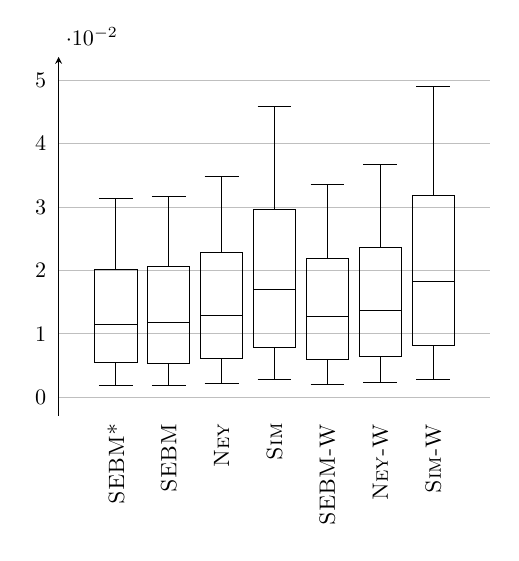
\begin{tikzpicture}[scale=0.8]
				\begin{axis}[
				boxplot/draw direction=y,
				x axis line style={opacity=0},
				y axis line style={opacity=10},
				tick style={opacity=0},
				%xticklabel style={opacity=0},
				axis x line*=bottom,
				axis y line=left,
				enlarge y limits,
				ymajorgrids,
				xtick={1,2,3,4,5,6,7},
				xticklabels={
					\STAB{\rotatebox[origin=c]{90}{\textsc{SEBM*}}}, 
					\STAB{\rotatebox[origin=c]{90}{\textsc{SEBM}}},
					\STAB{\rotatebox[origin=c]{90}{\textsc{Ney}}},
					\STAB{\rotatebox[origin=c]{90}{\textsc{Sim}}},
					\STAB{\rotatebox[origin=c]{90}{\textsc{SEBM-W}}},
					\STAB{\rotatebox[origin=c]{90}{\textsc{Ney-W}}},
					\STAB{\rotatebox[origin=c]{90}{\textsc{Sim-W}}},
					},
				]
\addplot [boxplot prepared={ 	lower whisker=0.0018873442,	lower quartile=0.0054911707,	median=0.0115660651,	upper quartile=0.0201957067,	upper whisker=0.0313351194 }] coordinates {};
\addplot [boxplot prepared={ 	lower whisker=0.0018479678,	lower quartile=0.0053737763,	median=0.0118668377,	upper quartile=0.0206569562,	upper whisker=0.0317171693 }] coordinates {};
\addplot [boxplot prepared={ 	lower whisker=0.0021922008,	lower quartile=0.0061725579,	median=0.0129446214,	upper quartile=0.0227833654,	upper whisker=0.0347607822 }] coordinates {};
\addplot [boxplot prepared={ 	lower whisker=0.0028718562,	lower quartile=0.0079247612,	median=0.0169270709,	upper quartile=0.0295933780,	upper whisker=0.0459081666 }] coordinates {};
\addplot [boxplot prepared={ 	lower whisker=0.0020786809,	lower quartile=0.0060284247,	median=0.0128084095,	upper quartile=0.0218762979,	upper whisker=0.0335333484 }] coordinates {};
\addplot [boxplot prepared={ 	lower whisker=0.0024134443,	lower quartile=0.0064584596,	median=0.0137104514,	upper quartile=0.0236670376,	upper whisker=0.0366193152 }] coordinates {};
\addplot [boxplot prepared={ 	lower whisker=0.0029029450,	lower quartile=0.0081964704,	median=0.0182601656,	upper quartile=0.0317369767,	upper whisker=0.0489318088 }] coordinates {};
				\end{axis}
			\end{tikzpicture}
		\end{tabular}
    \end{subfigure}%
    ~ 
    \begin{subfigure}[t]{0.5\textwidth}
        \centering
        \caption{$50N$ Samples}
        \begin{tabular}{m{79mm}}
			%\STAB{\rotatebox[origin=c]{90}{Absolute error}}  & 
			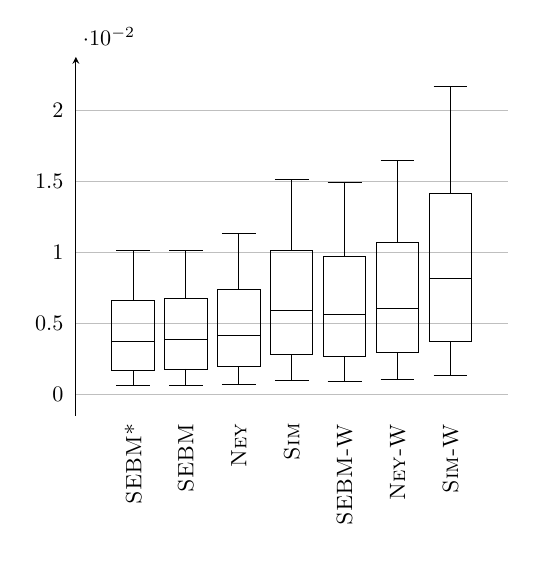
\begin{tikzpicture}[scale=0.8]
				\begin{axis}[
				boxplot/draw direction=y,
				x axis line style={opacity=0},
				y axis line style={opacity=10},
				tick style={opacity=0},
				%xticklabel style={opacity=0},
				axis x line*=bottom,
				axis y line=left,
				enlarge y limits,
				ymajorgrids,
				xtick={1,2,3,4,5,6,7},
				xticklabels={
					\STAB{\rotatebox[origin=c]{90}{\textsc{SEBM*}}}, 
					\STAB{\rotatebox[origin=c]{90}{\textsc{SEBM}}},
					\STAB{\rotatebox[origin=c]{90}{\textsc{Ney}}},
					\STAB{\rotatebox[origin=c]{90}{\textsc{Sim}}},
					\STAB{\rotatebox[origin=c]{90}{\textsc{SEBM-W}}},
					\STAB{\rotatebox[origin=c]{90}{\textsc{Ney-W}}},
					\STAB{\rotatebox[origin=c]{90}{\textsc{Sim-W}}},
					},
				]
\addplot [boxplot prepared={ 	lower whisker=0.0006317745,	lower quartile=0.0017075651,	median=0.0037366819,	upper quartile=0.0066579256,	upper whisker=0.0101485243 }] coordinates {};
\addplot [boxplot prepared={ 	lower whisker=0.0006254570,	lower quartile=0.0018023616,	median=0.0038633230,	upper quartile=0.0067541034,	upper whisker=0.0101255761 }] coordinates {};
\addplot [boxplot prepared={ 	lower whisker=0.0007068025,	lower quartile=0.0019893738,	median=0.0041560744,	upper quartile=0.0074129385,	upper whisker=0.0113558155 }] coordinates {};
\addplot [boxplot prepared={ 	lower whisker=0.0009682683,	lower quartile=0.0028052432,	median=0.0058995027,	upper quartile=0.0101560274,	upper whisker=0.0151640754 }] coordinates {};
\addplot [boxplot prepared={ 	lower whisker=0.0009266727,	lower quartile=0.0027205398,	median=0.0056726952,	upper quartile=0.0097018076,	upper whisker=0.0149751711 }] coordinates {};
\addplot [boxplot prepared={ 	lower whisker=0.0010340062,	lower quartile=0.0029374901,	median=0.0061035944,	upper quartile=0.0107265593,	upper whisker=0.0165181205 }] coordinates {};
\addplot [boxplot prepared={ 	lower whisker=0.0013318739,	lower quartile=0.0037411720,	median=0.0082145154,	upper quartile=0.0141625267,	upper whisker=0.0216969056 }] coordinates {};
				\end{axis}
			\end{tikzpicture}
		\end{tabular}
    \end{subfigure}
    ~\\
    \begin{subfigure}[t]{0.5\textwidth}
        \centering
        \caption{$100N$ Samples}
        \begin{tabular}{m{79mm}}
			%\STAB{\rotatebox[origin=c]{90}{Absolute error}}  & 
			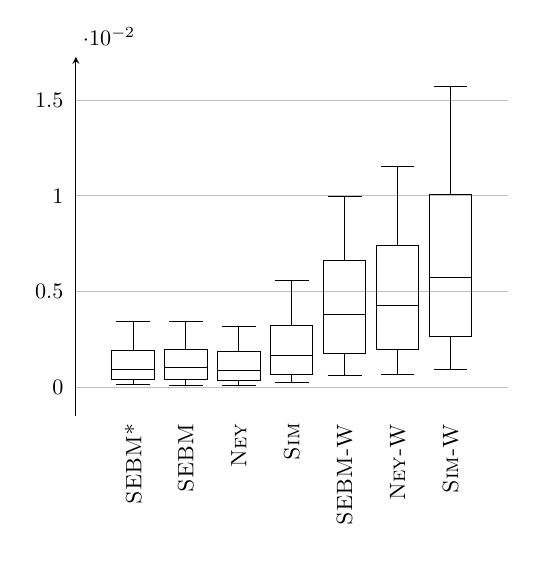
\begin{tikzpicture}[scale=0.8]
				\begin{axis}[
				boxplot/draw direction=y,
				x axis line style={opacity=0},
				y axis line style={opacity=10},
				tick style={opacity=0},
				%xticklabel style={opacity=0},
				axis x line*=bottom,
				axis y line=left,
				enlarge y limits,
				ymajorgrids,
				xtick={1,2,3,4,5,6,7},
				xticklabels={
					\STAB{\rotatebox[origin=c]{90}{\textsc{SEBM*}}}, 
					\STAB{\rotatebox[origin=c]{90}{\textsc{SEBM}}},
					\STAB{\rotatebox[origin=c]{90}{\textsc{Ney}}},
					\STAB{\rotatebox[origin=c]{90}{\textsc{Sim}}},
					\STAB{\rotatebox[origin=c]{90}{\textsc{SEBM-W}}},
					\STAB{\rotatebox[origin=c]{90}{\textsc{Ney-W}}},
					\STAB{\rotatebox[origin=c]{90}{\textsc{Sim-W}}},
					},
				]
\addplot [boxplot prepared={ 	lower whisker=0.0001280885,	lower quartile=0.0004091609,	median=0.0009608992,	upper quartile=0.0019509338,	upper whisker=0.0034539464 }] coordinates {};
\addplot [boxplot prepared={ 	lower whisker=0.0001214929,	lower quartile=0.0004127442,	median=0.0010239277,	upper quartile=0.0019695187,	upper whisker=0.0034196308 }] coordinates {};
\addplot [boxplot prepared={ 	lower whisker=0.0000887940,	lower quartile=0.0003453961,	median=0.0009018108,	upper quartile=0.0018647632,	upper whisker=0.0032042007 }] coordinates {};
\addplot [boxplot prepared={ 	lower whisker=0.0002323793,	lower quartile=0.0007009104,	median=0.0016518310,	upper quartile=0.0032361165,	upper whisker=0.0055755819 }] coordinates {};
\addplot [boxplot prepared={ 	lower whisker=0.0006414256,	lower quartile=0.0017828457,	median=0.0037858308,	upper quartile=0.0066402593,	upper whisker=0.0099905951 }] coordinates {};
\addplot [boxplot prepared={ 	lower whisker=0.0006944519,	lower quartile=0.0019705222,	median=0.0042941941,	upper quartile=0.0074174513,	upper whisker=0.0115165138 }] coordinates {};
\addplot [boxplot prepared={ 	lower whisker=0.0009351839,	lower quartile=0.0026407413,	median=0.0057360097,	upper quartile=0.0100919555,	upper whisker=0.0157014205 }] coordinates {};
				\end{axis}
			\end{tikzpicture}
		\end{tabular}
    \end{subfigure}%
    ~ 
    \begin{subfigure}[t]{0.5\textwidth}
        \centering
        \caption{$150N$ Samples}
        \begin{tabular}{m{79mm}}
			%\STAB{\rotatebox[origin=c]{90}{Absolute error}}  & 
			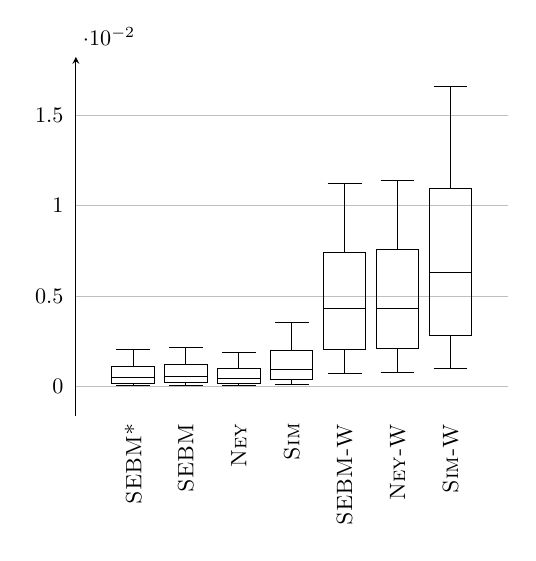
\begin{tikzpicture}[scale=0.8]
				\begin{axis}[
				boxplot/draw direction=y,
				x axis line style={opacity=0},
				y axis line style={opacity=10},
				tick style={opacity=0},
				%xticklabel style={opacity=0},
				axis x line*=bottom,
				axis y line=left,
				enlarge y limits,
				ymajorgrids,
				xtick={1,2,3,4,5,6,7},
				xticklabels={
					\STAB{\rotatebox[origin=c]{90}{\textsc{SEBM*}}}, 
					\STAB{\rotatebox[origin=c]{90}{\textsc{SEBM}}},
					\STAB{\rotatebox[origin=c]{90}{\textsc{Ney}}},
					\STAB{\rotatebox[origin=c]{90}{\textsc{Sim}}},
					\STAB{\rotatebox[origin=c]{90}{\textsc{SEBM-W}}},
					\STAB{\rotatebox[origin=c]{90}{\textsc{Ney-W}}},
					\STAB{\rotatebox[origin=c]{90}{\textsc{Sim-W}}},
					},
				]
\addplot [boxplot prepared={ 	lower whisker=0.0000487139,	lower quartile=0.0001863473,	median=0.0005003290,	upper quartile=0.0011015025,	upper whisker=0.002037994 }] coordinates {};
\addplot [boxplot prepared={ 	lower whisker=0.0000441026,	lower quartile=0.0002008982,	median=0.0005643273,	upper quartile=0.0012115181,	upper whisker=0.0021373138 }] coordinates {};
\addplot [boxplot prepared={ 	lower whisker=0.0000365317,	lower quartile=0.0001551298,	median=0.0004437645,	upper quartile=0.0009719484,	upper whisker=0.0018915558 }] coordinates {};
\addplot [boxplot prepared={ 	lower whisker=0.0001207363,	lower quartile=0.0004074072,	median=0.0009602551,	upper quartile=0.0019643373,	upper whisker=0.0035355047 }] coordinates {};
\addplot [boxplot prepared={ 	lower whisker=0.0006971353,	lower quartile=0.0020289290,	median=0.0043020196,	upper quartile=0.0074356075,	upper whisker=0.0112135668 }] coordinates {};
\addplot [boxplot prepared={ 	lower whisker=0.0007556367,	lower quartile=0.0020795855,	median=0.0043218693,	upper quartile=0.0075658289,	upper whisker=0.011420641 }] coordinates {};
\addplot [boxplot prepared={ 	lower whisker=0.0010075904,	lower quartile=0.0027975286,	median=0.0063083297,	upper quartile=0.0109494123,	upper whisker=0.0165960243 }] coordinates {};
				\end{axis}
			\end{tikzpicture}
		\end{tabular}
    \end{subfigure}
    \caption{Distribution of numerical absolute errors across 5000 rounds of beta-distributed data, for different methods of stratified sampling. 
    Each plot shows absolute errors for different numbers of samples multiplied by the number of strata, $N$, e.g. $10N$ samples means that the test problem has a sample budget of ten times the number of strata. The whiskers show the 9th and 91st percentiles, data points outside this range are not shown.}
\label{Table1}
\end{figure*}


\begin{figure*}[hbtp]
    \centering
    \begin{subfigure}[t]{0.5\textwidth}
        \centering
        \caption{$10N$ Samples}
        \begin{tabular}{m{79mm}}
			%\STAB{\rotatebox[origin=c]{90}{Absolute error}}  & 
			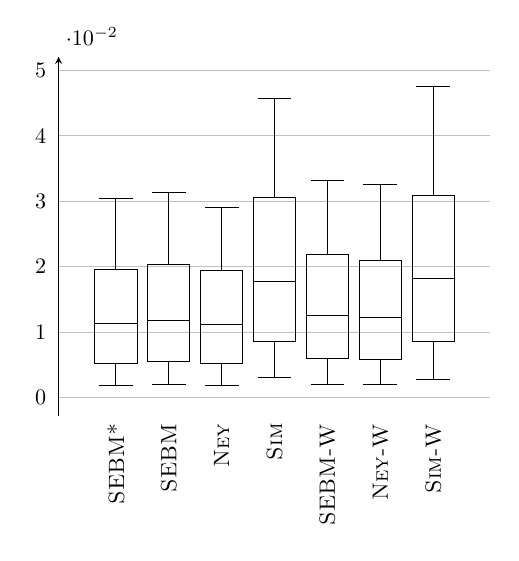
\begin{tikzpicture}[scale=0.8]
				\begin{axis}[
				boxplot/draw direction=y,
				x axis line style={opacity=0},
				y axis line style={opacity=10},
				tick style={opacity=0},
				%xticklabel style={opacity=0},
				axis x line*=bottom,
				axis y line=left,
				enlarge y limits,
				ymajorgrids,
				xtick={1,2,3,4,5,6,7},
				xticklabels={
					\STAB{\rotatebox[origin=c]{90}{\textsc{SEBM*}}}, 
					\STAB{\rotatebox[origin=c]{90}{\textsc{SEBM}}},
					\STAB{\rotatebox[origin=c]{90}{\textsc{Ney}}},
					\STAB{\rotatebox[origin=c]{90}{\textsc{Sim}}},
					\STAB{\rotatebox[origin=c]{90}{\textsc{SEBM-W}}},
					\STAB{\rotatebox[origin=c]{90}{\textsc{Ney-W}}},
					\STAB{\rotatebox[origin=c]{90}{\textsc{Sim-W}}},
					},
				]
\addplot [boxplot prepared={ 	lower whisker=0.00183620673831,	lower quartile=0.00529326798954,	median=0.0113256580991,	upper quartile=0.0196658708913,	upper whisker=0.0304730202339 }] coordinates {};
\addplot [boxplot prepared={ 	lower whisker=0.00195844950636,	lower quartile=0.00548889744201,	median=0.0117513166962,	upper quartile=0.0203418348306,	upper whisker=0.0314299792713 }] coordinates {};
\addplot [boxplot prepared={ 	lower whisker=0.00185260938009,	lower quartile=0.00527319771539,	median=0.0112495148219,	upper quartile=0.0194023114891,	upper whisker=0.0290303015612 }] coordinates {};
\addplot [boxplot prepared={ 	lower whisker=0.00301932237342,	lower quartile=0.00859135974251,	median=0.017721270595,	upper quartile=0.0305333890174,	upper whisker=0.0456908434243 }] coordinates {};
\addplot [boxplot prepared={ 	lower whisker=0.00197845370017,	lower quartile=0.00595378784258,	median=0.012575753413,	upper quartile=0.0218576520232,	upper whisker=0.033261552165 }] coordinates {};
\addplot [boxplot prepared={ 	lower whisker=0.00209628378338,	lower quartile=0.00586974191243,	median=0.0122918680826,	upper quartile=0.0209279090071,	upper whisker=0.0326546061431 }] coordinates {};
\addplot [boxplot prepared={ 	lower whisker=0.002836019658,	lower quartile=0.00853787778199,	median=0.0181510463289,	upper quartile=0.0309749413241,	upper whisker=0.047509682599 }] coordinates {};
				\end{axis}
			\end{tikzpicture}
		\end{tabular}
    \end{subfigure}%
    ~ 
    \begin{subfigure}[t]{0.5\textwidth}
        \centering
        \caption{$50N$ Samples}
        \begin{tabular}{m{79mm}}
			%\STAB{\rotatebox[origin=c]{90}{Absolute error}}  & 
			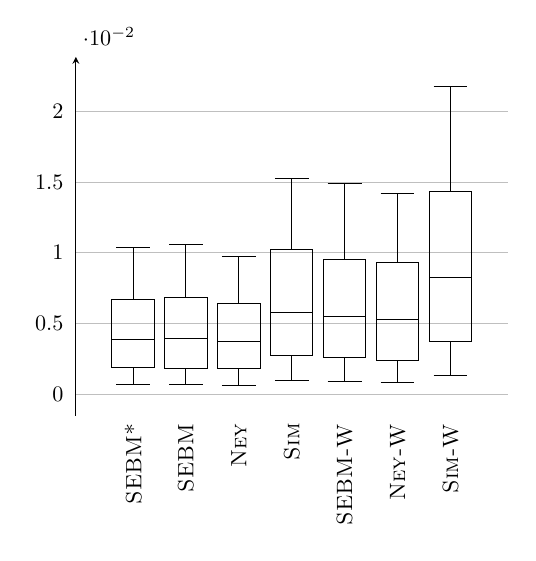
\begin{tikzpicture}[scale=0.8]
				\begin{axis}[
				boxplot/draw direction=y,
				x axis line style={opacity=0},
				y axis line style={opacity=10},
				tick style={opacity=0},
				%xticklabel style={opacity=0},
				axis x line*=bottom,
				axis y line=left,
				enlarge y limits,
				ymajorgrids,
				xtick={1,2,3,4,5,6,7},
				xticklabels={
					\STAB{\rotatebox[origin=c]{90}{\textsc{SEBM*}}}, 
					\STAB{\rotatebox[origin=c]{90}{\textsc{SEBM}}},
					\STAB{\rotatebox[origin=c]{90}{\textsc{Ney}}},
					\STAB{\rotatebox[origin=c]{90}{\textsc{Sim}}},
					\STAB{\rotatebox[origin=c]{90}{\textsc{SEBM-W}}},
					\STAB{\rotatebox[origin=c]{90}{\textsc{Ney-W}}},
					\STAB{\rotatebox[origin=c]{90}{\textsc{Sim-W}}},
					},
				]
\addplot [boxplot prepared={ 	lower whisker=0.000686690622579,	lower quartile=0.00186362339474,	median=0.00386518148388,	upper quartile=0.00666698900838,	upper whisker=0.0103445166593 }] coordinates {};
\addplot [boxplot prepared={ 	lower whisker=0.000656830615007,	lower quartile=0.00182143598221,	median=0.00396566843382,	upper quartile=0.00684716409054,	upper whisker=0.0106033374063 }] coordinates {};
\addplot [boxplot prepared={ 	lower whisker=0.000596050228624,	lower quartile=0.00178770145456,	median=0.00374572449749,	upper quartile=0.00638952219117,	upper whisker=0.00972678199143 }] coordinates {};
\addplot [boxplot prepared={ 	lower whisker=0.000962495646602,	lower quartile=0.00274422909247,	median=0.00578715807377,	upper quartile=0.0101983818534,	upper whisker=0.015234872938 }] coordinates {};
\addplot [boxplot prepared={ 	lower whisker=0.000924496690244,	lower quartile=0.00257957242393,	median=0.00548964169828,	upper quartile=0.00954969321953,	upper whisker=0.0148981942896 }] coordinates {};
\addplot [boxplot prepared={ 	lower whisker=0.000842005939279,	lower quartile=0.00238425788913,	median=0.00531315213905,	upper quartile=0.00930113789744,	upper whisker=0.0141974030969 }] coordinates {};
\addplot [boxplot prepared={ 	lower whisker=0.00128572549222,	lower quartile=0.00373034258211,	median=0.00823497231891,	upper quartile=0.0143440178995,	upper whisker=0.0217365923271 }] coordinates {};
				\end{axis}
			\end{tikzpicture}
		\end{tabular}
    \end{subfigure}
    ~\\
    \begin{subfigure}[t]{0.5\textwidth}
        \centering
        \caption{$100N$ Samples}
        \begin{tabular}{m{79mm}}
			%\STAB{\rotatebox[origin=c]{90}{Absolute error}}  & 
			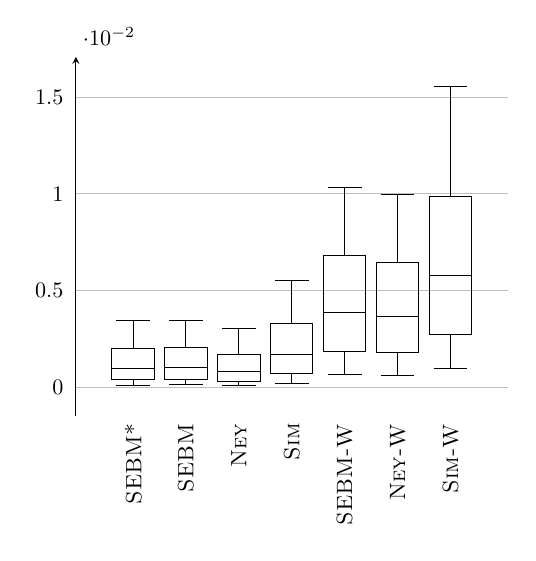
\begin{tikzpicture}[scale=0.8]
				\begin{axis}[
				boxplot/draw direction=y,
				x axis line style={opacity=0},
				y axis line style={opacity=10},
				tick style={opacity=0},
				%xticklabel style={opacity=0},
				axis x line*=bottom,
				axis y line=left,
				enlarge y limits,
				ymajorgrids,
				xtick={1,2,3,4,5,6,7},
				xticklabels={
					\STAB{\rotatebox[origin=c]{90}{\textsc{SEBM*}}}, 
					\STAB{\rotatebox[origin=c]{90}{\textsc{SEBM}}},
					\STAB{\rotatebox[origin=c]{90}{\textsc{Ney}}},
					\STAB{\rotatebox[origin=c]{90}{\textsc{Sim}}},
					\STAB{\rotatebox[origin=c]{90}{\textsc{SEBM-W}}},
					\STAB{\rotatebox[origin=c]{90}{\textsc{Ney-W}}},
					\STAB{\rotatebox[origin=c]{90}{\textsc{Sim-W}}},
					},
				]
\addplot [boxplot prepared={ 	lower whisker=0.000124161859425,	lower quartile=0.000414925714979,	median=0.00100282029566,	upper quartile=0.0019866547283,	upper whisker=0.00344859203723 }] coordinates {};
\addplot [boxplot prepared={ 	lower whisker=0.000138979541446,	lower quartile=0.000434668312365,	median=0.00103459291697,	upper quartile=0.0020634398688,	upper whisker=0.00346804389981 }] coordinates {};
\addplot [boxplot prepared={ 	lower whisker=0.0000884130547408,	lower quartile=0.000324331846734,	median=0.000818171087152,	upper quartile=0.0017061867139,	upper whisker=0.00307006681596 }] coordinates {};
\addplot [boxplot prepared={ 	lower whisker=0.000227015098149,	lower quartile=0.000708726110964,	median=0.00167649650203,	upper quartile=0.00332448862188,	upper whisker=0.00555099763664 }] coordinates {};
\addplot [boxplot prepared={ 	lower whisker=0.000678454797763,	lower quartile=0.00184394817862,	median=0.00389438997983,	upper quartile=0.00682031670303,	upper whisker=0.0103532251521 }] coordinates {};
\addplot [boxplot prepared={ 	lower whisker=0.000636466511201,	lower quartile=0.00178306753911,	median=0.00365955369572,	upper quartile=0.00645314643273,	upper whisker=0.00996489319949 }] coordinates {};
\addplot [boxplot prepared={ 	lower whisker=0.000955905266177,	lower quartile=0.00273954329606,	median=0.00577716505587,	upper quartile=0.00987599743817,	upper whisker=0.0155387629673 }] coordinates {};
				\end{axis}
			\end{tikzpicture}
		\end{tabular}
    \end{subfigure}%
    ~ 
    \begin{subfigure}[t]{0.5\textwidth}
        \centering
        \caption{$150N$ Samples}
        \begin{tabular}{m{79mm}}
			%\STAB{\rotatebox[origin=c]{90}{Absolute error}}  & 
			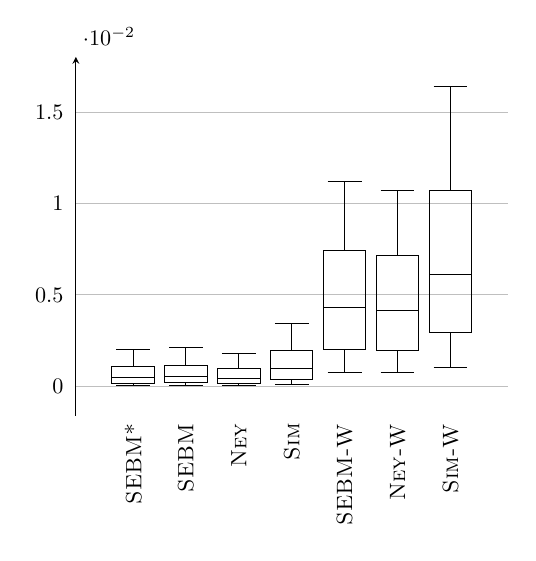
\begin{tikzpicture}[scale=0.8]
				\begin{axis}[
				boxplot/draw direction=y,
				x axis line style={opacity=0},
				y axis line style={opacity=10},
				tick style={opacity=0},
				%xticklabel style={opacity=0},
				axis x line*=bottom,
				axis y line=left,
				enlarge y limits,
				ymajorgrids,
				xtick={1,2,3,4,5,6,7},
				xticklabels={
					\STAB{\rotatebox[origin=c]{90}{\textsc{SEBM*}}}, 
					\STAB{\rotatebox[origin=c]{90}{\textsc{SEBM}}},
					\STAB{\rotatebox[origin=c]{90}{\textsc{Ney}}},
					\STAB{\rotatebox[origin=c]{90}{\textsc{Sim}}},
					\STAB{\rotatebox[origin=c]{90}{\textsc{SEBM-W}}},
					\STAB{\rotatebox[origin=c]{90}{\textsc{Ney-W}}},
					\STAB{\rotatebox[origin=c]{90}{\textsc{Sim-W}}},
					},
				]
\addplot [boxplot prepared={ 	lower whisker=0.0000471307005487,	lower quartile=0.000180612998704,	median=0.000495999100557,	upper quartile=0.00109741530852,	upper whisker=0.00202850157066 }] coordinates {};
\addplot [boxplot prepared={ 	lower whisker=0.0000522578790047,	lower quartile=0.000201132599965,	median=0.000539735990992,	upper quartile=0.00115797688066,	upper whisker=0.00211349682588 }] coordinates {};
\addplot [boxplot prepared={ 	lower whisker=0.0000352347557525,	lower quartile=0.000147554764468,	median=0.000419518785648,	upper quartile=0.000958045623416,	upper whisker=0.00180090868101 }] coordinates {};
\addplot [boxplot prepared={ 	lower whisker=0.000118052373968,	lower quartile=0.000396135405203,	median=0.000987226504158,	upper quartile=0.00195355411425,	upper whisker=0.0034476280125 }] coordinates {};
\addplot [boxplot prepared={ 	lower whisker=0.000755387160653,	lower quartile=0.00202006161526,	median=0.00434133400793,	upper quartile=0.00744880448204,	upper whisker=0.0112240543617 }] coordinates {};
\addplot [boxplot prepared={ 	lower whisker=0.00073454521555,	lower quartile=0.00196916707916,	median=0.0041427938489,	upper quartile=0.00717740309752,	upper whisker=0.0107154595421 }] coordinates {};
\addplot [boxplot prepared={ 	lower whisker=0.0010523697351,	lower quartile=0.00295840792712,	median=0.00614543093609,	upper quartile=0.0107394289896,	upper whisker=0.0163908256951 }] coordinates {};
				\end{axis}
			\end{tikzpicture}
		\end{tabular}
    \end{subfigure}
    \caption{Distribution of numerical absolute errors across 5000 rounds of beta-distributed data, for different methods of stratified sampling. 
    Each plot shows absolute errors for different numbers of samples multiplied by the number of strata, $N$, e.g. $10N$ samples means that the test problem has a sample budget of ten times the number of strata. The whiskers show the 9th and 91st percentiles, data points outside this range are not shown.}
\label{Table1}
\end{figure*}


Figure \ref{Table1} compares the distribution of absolute error achieved by each of the sampling methods over 5000 rounds of these data sets.
Each panel presents the results that the methods achieve for a given budget of samples, 
expressed as a multiple of the number of strata (noting that data sets where the sampling budget exceeded the volume of data were excluded).
From the plots in Figure \ref{Table1}, we can see that our sampling technique (SEBM and SEBM-W) performs comparably to
% competitive-to and sometimes better-than 
Neyman sampling (\textsc{Ney} and \textsc{Ney-W}) despite not having access to knowledge of stratum variances.
Also, there is a notable similarity between SEBM* and SEBM.
As expected, sampling without replacement always performs better than sampling with replacement for the same method, and this difference is magnified as the number of samples grows large in comparison to the population size. 
Finally, simple random sampling almost always performs worst, because it fails to take advantage of any variance information.
These results and their interpretation are discussed and detailed in Section~\ref{sec:discussion} along with results from the other test cases discussed below.



\subsubsection{A Uniform and Bernoulli Distribution}
\label{sec:dataset2}
The aim of this section is to examine cases of distributions in which our sampling method (SEBM) performs poorly, particularly compared to Neyman sampling (\textsc{Ney}).
For this purpose, a data set with two strata is generated, with each stratum containing $1000$ points. 
The data in the first stratum is uniform continuous data in range $[0,1]$, while the data in the second is Bernoulli distributed, with all zeros except for a specified small number, $a$, of successes with value 1.
For this problem, we conduct stratified random sampling with a budget of $300$ samples, comparing the SEBM*, SEBM and \textsc{Ney} methods.
The average error returned by the methods across 20,000 realizations of this problem, plotted against the number of successes $a$, are shown as a graph in Figure \ref{biggraph3}.

This figure demonstrates that SEBM and SEBM* perform poorly when the strata contain only very small numbers of successes.
This under-performance is not simply a result of the SEBM method oversampling in a process of learning the stratum variances, as the under-performance is present in SEBM* as well.
The reasons for this under-performance are discussed in conjunction with other results in more detail in Section~\ref{sec:discussion}.
Before this, we considered the calculation of the Shapley value as an example computational application of our stratified sampling method.

%\begin{figure}[ht]
	\centering
	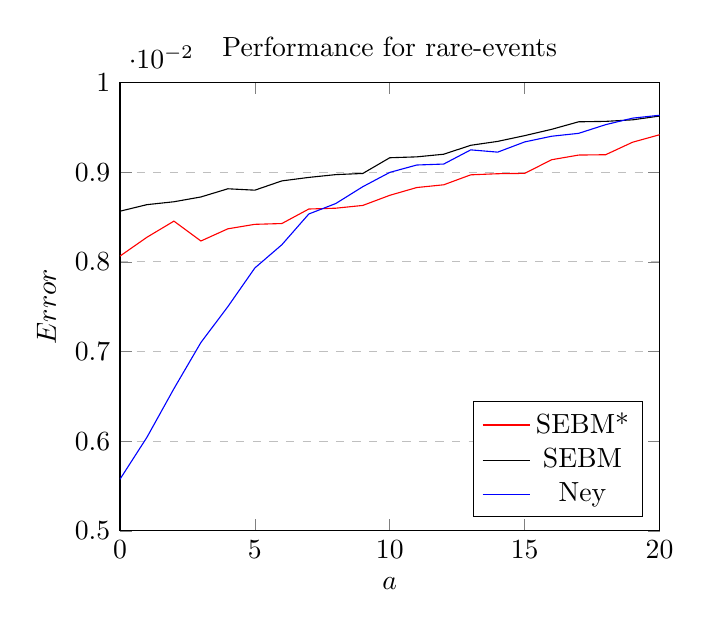
\begin{tikzpicture}[scale=1.0]
		\begin{axis}[
			title={Performance for rare-events},
			xlabel={$a$},
			xmin=0, xmax=20,
			ymin=0.005, ymax=0.01,
			ymajorgrids=true,
			ylabel={$Error$},
			grid style=dashed,
			xticklabel style={/pgf/number format/fixed},
			legend pos=south east,
		]
		\addplot[color=red] coordinates {
		(0, 0.00806368)(1, 0.00827372)(2, 0.00845386)(3, 0.00823214)(4, 0.00836828)(5, 0.00841808)(6, 0.00842695)(7, 0.00858889)(8, 0.00859801)(9, 0.00862887)(10, 0.00874168)(11, 0.00882848)(12, 0.00885912)(13, 0.00897012)(14, 0.00898256)(15, 0.0089864)(16, 0.00913864)(17, 0.00919064)(18, 0.00919448)(19, 0.00933398)(20, 0.00941723)(21, 0.00936993)(22, 0.00937978)(23, 0.00955662)(24, 0.00950003)(25, 0.00961189)(26, 0.0097152)(27, 0.00970903)(28, 0.00976764)(29, 0.0097812)(30, 0.00989442)
		};
\addlegendentry{SEBM*}
		\addplot[] coordinates {
		(0, 0.00856433)(1, 0.00863755)(2, 0.00866977)(3, 0.00872333)(4, 0.00881456)(5, 0.00879907)(6, 0.00890246)(7, 0.00894146)(8, 0.00897258)(9, 0.00898535)(10, 0.00916068)(11, 0.00917059)(12, 0.00919994)(13, 0.00929965)(14, 0.00934318)(15, 0.00940736)(16, 0.00947778)(17, 0.00956169)(18, 0.00956631)(19, 0.00958364)(20, 0.00962582)(21, 0.00962475)(22, 0.00973724)(23, 0.00975617)(24, 0.00981378)(25, 0.00984651)(26, 0.00990438)(27, 0.00994233)(28, 0.00992333)(29, 0.0100455)(30, 0.0101047)
		};
\addlegendentry{SEBM}
		\addplot[color=blue] coordinates {
		(0, 0.00557472)(1, 0.00604282)(2, 0.00658481)(3, 0.00709998)(4, 0.00750014)(5, 0.00793152)(6, 0.00819032)(7, 0.0085335)(8, 0.00865024)(9, 0.00883771)(10, 0.00899734)(11, 0.0090796)(12, 0.00909045)(13, 0.00924854)(14, 0.00922326)(15, 0.00933714)(16, 0.0094006)(17, 0.00943286)(18, 0.00952964)(19, 0.00960244)(20, 0.0096347)(21, 0.00964669)(22, 0.00963958)(23, 0.00974312)(24, 0.00977512)(25, 0.00985768)(26, 0.00991623)(27, 0.00999059)(28, 0.00985384)(29, 0.00997242)(30, 0.0100606)
		};
\addlegendentry{Ney}
		\end{axis}
	\end{tikzpicture}
    \caption{Average error of three stratified random sampling methods for the uniform-Bernoulli data sets of Section~\ref{sec:dataset2}, plotted against success parameter $a$, across 20,000 rounds.}
	\label{biggraph3}
\end{figure}

\begin{figure}[ht]
	\centering
	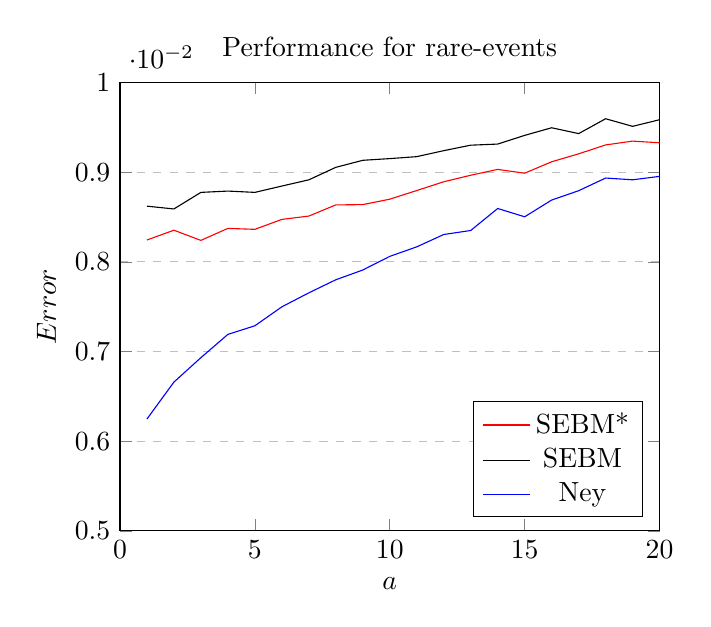
\begin{tikzpicture}[scale=1.0]
		\begin{axis}[
			title={Performance for rare-events},
			xlabel={$a$},
			xmin=0, xmax=20,
			ymin=0.005, ymax=0.01,
			ymajorgrids=true,
			ylabel={$Error$},
			grid style=dashed,
			xticklabel style={/pgf/number format/fixed},
			legend pos=south east,
		]
		\addplot[color=red] coordinates {
		(1,0.00824303292213)(2,0.00835254460775)(3,0.00823889901958)(4,0.00837282775519)(5,0.00836224382102)(6,0.00847304546572)(7,0.00851017908833)(8,0.00863460077097)(9,0.00863804338539)(10,0.00869846985716)(11,0.00879500733656)(12,0.00889282803455)(13,0.00896565747936)(14,0.00903077609739)(15,0.0089882646374)(16,0.00911591098473)(17,0.00920413707689)(18,0.00930364609753)(19,0.00934625157477)(20,0.0093274509829)
		};
\addlegendentry{SEBM*}
		\addplot[] coordinates {
		(1,0.00862069641015)(2,0.00858955811405)(3,0.0087743808877)(4,0.00878901680047)(5,0.00877444275485)(6,0.00884487890096)(7,0.00891432838845)(8,0.00905367745213)(9,0.00913216007212)(10,0.00915117512012)(11,0.0091729326627)(12,0.00923976838734)(13,0.00930083022747)(14,0.00931320531153)(15,0.00941021263061)(16,0.00949516652951)(17,0.00942991982115)(18,0.00959562689618)(19,0.00951087083342)(20,0.00958483466397)
		};
\addlegendentry{SEBM}
		\addplot[color=blue] coordinates {
		(1,0.00624623729428)(2,0.00665878512663)(3,0.00693118423385)(4,0.00719049815418)(5,0.00728657163073)(6,0.0074977146605)(7,0.00765404831751)(8,0.00779979414445)(9,0.00790867351491)(10,0.00806086399739)(11,0.00816687885093)(12,0.00830452351902)(13,0.00834938001649)(14,0.00859465863069)(15,0.0085021791087)(16,0.00868887793215)(17,0.0087930307321)(18,0.0089343323971)(19,0.00891468625456)(20,0.00895299850251)
		};
\addlegendentry{Ney}
		\end{axis}
	\end{tikzpicture}
    \caption{Average error of three stratified random sampling methods for the uniform-Bernoulli data sets of Section~\ref{sec:dataset2}, plotted against success parameter $a$, across 20,000 rounds.}
	\label{biggraph3}
\end{figure}


\section{Shapley Value Approximation}\label{sec:shapley}

The Shapley value is a cornerstone measure in cooperative game theory. 
It is an axiomatic approach to allocating a divisible reward or cost between participants where there is a clearly defined notion of how much surplus or profit a group or ``coalition'' of participants could achieve by themselves \citep{ChalkiadakisEtAl2012}.
It has many applications, 
including analyzing the power of voting blocks in weighted voting games \citep{Bachrach2009ApproximatingPI}, 
in cost and surplus division problems  \citep{AzizEtal2016,archie_paper1}, 
and as a measure of network centrality \citep{Michalak:2013}.

Formally, a \textit{cooperative game}, $\langle N,v\rangle\in\mathbb{G}_N$, comprises a set of $n$ players, $N=\{1,2,\dots,n\}$, and a \textit{characteristic function}, $v:S\subset N\rightarrow \mathbb{R}$, which is a function specifying the reward which can be achieved if a subset of the players $S\subset N$ cooperate, where $v(\emptyset)=0$.
In this context the Shapley value $\varphi$ is a unique mapping from cooperative games to the player rewards $\mathbb{G}_N\rightarrow\mathbb{R}^n$ which satisfies axioms:

\begin{itemize}
\item	
\textbf{Efficiency}: That the total reward is divided up: $\sum_i\varphi_i(\langle N,v\rangle) = v(N)$
\item	
\textbf{Symmetry}: If two players $i$ and $j$ are totally equivalent `substitutes' then the receive the same reward: ie. if $v(S\cup i)=v(S\cup j)~~\forall S\subseteq N\setminus\{i,j\}$, then $\varphi_i(\langle N,v\rangle) = \varphi_i(\langle N,v\rangle)$
\item	
\textbf{Null Player}: If the addition of a player $i$ to any coalition brings nothing, and is a `null player', then it receives reward of zero: i.e if $v(S\cup i)=v(S)~~\forall S\subseteq N$ then $\varphi_i(\langle N,v\rangle)=0$
\item	
\textbf{Additivity}: That for any two games the reward afforded each player is each is the sum of the games considered together: i.e. for any $v_1$ and $v_2$, that: $\varphi(\langle N,v_1+v_2\rangle)=\varphi(\langle N,v_1 \rangle) + \varphi(\langle N,v_2\rangle)$
\end{itemize}

Specifically, the Shapley value is expressed as:
\begin{equation}\label{shap1}\varphi_i(\langle N,v\rangle) = \sum_{S\subset N, i\notin S}\frac{(n-|S|-1)!\,|S|!}{n!}(v(S\cup\{i\})-v(S))\end{equation}
That is, under the Shapley value each player is afforded their average marginal contribution across every possible sequence of player join orderings.  
Or, if $v_{i,k}$ is the average marginal contribution which player $i$ can make across coalitions of size $k$:
\begin{equation}
v_{i,k} = \frac{1}{\binom{n-1}{k}}\sum_{S\subset N\setminus \{ i\} , |S|=k} %\frac{(n-|S|-1)!\,|S|!}{(n-1)!}
(v(S\cup\{i\})-v(S))
\end{equation}
then the Shapley value can be expressed as an average:
\begin{equation}\label{shap2} \varphi_i(\langle N,v\rangle) = \frac{1}{n}\sum_{k=0}^{n-1}v_{i,k} \end{equation}
Though the Shapley value is conceptually simple, its use is hampered by the fact that its total expression involves exponentially many evaluations of the characteristic function (there are $n\times 2^{n-1}$ possible marginal contributions between $n$ players).

However, since the Shapley value is expressible as an average over averages by Equation~\eqref{shap2}, 
it is possible to approximate these averages via sampling techniques, and these averages are naturally stratified by coalition size.
In previously published literature, other techniques have been used to allocate samples in this context, particularly simple sampling \citep{DBLP:journals/cor/CastroGT09}, Neyman allocation \citep{CASTRO2017180,DBLP:journals/tsg/OBrienGR15}, and allocation to minimize Hoeffding's inequality \citep{2013arXiv1306.4265M}.

We assess the benefits of using our bound by comparing its performance to the approaches above in the context of some example cooperative games, with results analyzed in Section~\ref{sec:discussion}.
The example games are described below:

\begin{example_game}[Airport Game]
An $n=15$ player game with characteristic function:
$$v(S)=\max_{i\in S}w_i$$
where
$w=\{w_1,\dots,w_{15}\} %\scriptstyle\scriptsize
=\{ 1, 1, 2, 2, 2, 3, 4, 5, 5, 5, 7, 8, 8, 8, 10\}$.
The maximum marginal contribution is $10$, so we assign $D_i=10$ for all $i$.
\end{example_game}

\begin{example_game}[Voting Game]
An $n=15$ player game with characteristic function:
$$v(S)=\begin{cases}
       1, &\quad\text{if}\quad \sum_{i\in S}w_i>\sum_{j\in N}w_j/2\\
       0, &\quad\text{otherwise}\\
     \end{cases}$$
where 
$w=\{w_1,\dots,w_{15}\} %\scriptstyle\scriptsize
=\{ 1, 3, 3, 6, 12, 16, 17, 19, 19, 19, 21, 22, 23, 24, 29\}$.
The maximum marginal contribution is $1$, so we assign $D_i=1$ for all $i$.
\end{example_game}

\begin{example_game}[Simple Reward Division]
An $n=15$ player game with characteristic function:
$$v(S)=\frac{1}{2}\left(\sum_{i\in S}\frac{w_i}{100}\right)^2$$
where
$w=\{w_1,\dots,w_{15}\} = \{ 45, 41, 27, 26, 25, 21, 13, 13, 12, 12, 11, 11, 10, 10, 10 \}$\\
The maximum marginal contribution is $1.19025$, so we assign $D_i=1.19025$ for all $i$.
\end{example_game}

\begin{example_game}[Complex Reward Division]
An $n=15$ player game with characteristic function:
$$v(S)=\left(\sum_{i\in S}\frac{w_i}{50}\right)^2 - \floor[\Bigg]{\sum_{i\in S}\frac{w_i}{50}}^2$$
where
$w=\{w_1,\dots,w_{15}\} = \{ 45, 41, 27, 26, 25, 21, 13, 13, 12, 12, 11, 11, 10, 10, 10 \}$\\
In this game, we assign $D_i=2$ for all $i$.
\end{example_game}

%\begin{table*}[h]
    \centering 
    \begin{subfigure}[]{0.8\textwidth}
        \centering
        \caption{Airport Game Average Errors}\label{tab1}
			\begin{tabular}{llllll}
			\hline
			$\nicefrac{m}{n^2}$ & $10$ & $50$ & $100$ & $500$ & $1000$ \\
			\hline
			$e^{Ma}$   & 298.4 & 133.1 & 99.64 & 41.96 & 29.26 \\
			$e^{sim}$  & 357.8 & 146.1 & 106.2 & 44.55 & 36.33 \\
			$e^{Ca}$   & 325.7 & 115.8 & 75.85 & 31.01 & 22.12 \\
			$e^{SEBM}$ & 259.2 & 73.8 & 54.76 & 7.71 & 1.30  \\
			\hline
			\end{tabular}
    \end{subfigure}
	\\\vspace{4mm}
    \begin{subfigure}[]{0.8\textwidth}
        \centering
        \caption{Voting Game Average Errors}\label{tab2}
			\begin{tabular}{llllll}
			\hline
			$\nicefrac{m}{n^2}$ & $10$ & $50$ & $100$ & $500$ & $1000$ \\
			\hline
			$e^{Ma}$    & 131.0 & 57.78 & 41.52 & 18.66 & 13.18 \\
			$e^{sim}$   & 145.7 & 59.72 & 40.31 & 17.56 & 12.84 \\
			$e^{Ca}$    & 142.1 & 47.35 & 31.05 & 14.08 & 9.800 \\
			$e^{SEBM}$  & 122.8 & 47.44 & 33.18 & 8.55 & 1.995  \\
			\hline
			\end{tabular}
    \end{subfigure}
	\\\vspace{4mm}
    \begin{subfigure}[]{0.8\textwidth}
        \centering
        \caption{Simple Reward Division Game average errors}\label{tab3}
			\begin{tabular}{llllll}
			\hline
			$\nicefrac{m}{n^2}$ & $10$ & $50$ & $100$ & $500$ & $1000$ \\
			\hline
			$e^{Ma}$    & 25.68 & 11.62 & 7.792 & 3.481 & 2.290 \\
			$e^{sim}$   & 22.10 & 9.045 & 6.218 & 2.642 & 1.938 \\
			$e^{Ca}$    & 22.37 & 8.925 & 6.692 & 2.727 & 1.940 \\
			$e^{SEBM}$  & 19.25 & 7.044 & 5.158 & 1.183 & 0.2817  \\
			\hline
			\end{tabular}
    \end{subfigure}
	\\\vspace{4mm}
    \begin{subfigure}[]{0.8\textwidth}
        \centering
        \caption{Complex Reward Division Game average errors}\label{tab4}
			\centering
			\begin{tabular}{llllll}
			\hline
			$\nicefrac{m}{n^2}$ & $10$ & $50$ & $100$ & $500$ & $1000$ \\
			\hline
			$e^{Ma}$   & 276.1 & 118.9 & 87.00 & 40.15 & 27.44 \\
			$e^{sim}$  & 251.4 & 108.0 & 78.63 & 34.64 & 26.82 \\
			$e^{Ca}$   & 290.5 & 116.5 & 81.82 & 35.70 & 26.50 \\
			$e^{SEBM}$ & 214.2 & 78.47 & 54.10 & 12.45 & 2.711  \\
			\hline
			\end{tabular}
    \end{subfigure}
    \vspace{3mm}
    \caption{Average absolute errors in the Shapley value calculation across all players in the four cooperative games (units in $10^{-4}$), for the different sampling schemes with different sampling budgets $m$ per number of strata (with $n^2=15^2$ for all).}
    \label{Table2}
\end{table*}


%\begin{table*}[h]
%    \centering 
%    \begin{subfigure}[]{0.8\textwidth}
%        \centering
%        \caption{Airport Game average errors}\label{tab1}
%			\begin{tabular}{llllll}
%			\hline
%			$\nicefrac{m}{n^2}$ & $10$ & $50$ & $100$ & $500$ & $1000$ \\
%			\hline
%			$e^{Ma}$  & 298.36 & 133.07 & 99.639 & 41.963 & 29.257 \\
%			$e^{sim}$  & 357.84 & 146.09 & 106.22 & 44.545 & 36.333 \\
%			$e^{Ca}$  & 325.65 & 115.73 & 75.85 & 31.014 & 22.115 \\
%			$e^{SEBM}$  & 259.24 & 73.754 & 54.756 & 7.7099 & 1.3038  \\
%			\hline
%			\end{tabular}
%    \end{subfigure}
%	\\\vspace{4mm}
%    \begin{subfigure}[]{0.8\textwidth}
%        \centering
%        \caption{Voting Game average errors}\label{tab2}
%			\begin{tabular}{llllll}
%			\hline
%			$\nicefrac{m}{n^2}$ & $10$ & $50$ & $100$ & $500$ & $1000$ \\
%			\hline
%			$e^{Ma}$  & 130.98 & 57.775 & 41.522 & 18.657 & 13.178 \\
%			$e^{sim}$  & 145.72 & 59.716 & 40.306 & 17.563 & 12.835 \\
%			$e^{Ca}$  & 142.10 & 47.350 & 31.048 & 14.080 & 9.7998 \\
%			$e^{SEBM}$  & 122.79 & 47.435 & 33.179 & 8.5464 & 1.9953  \\
%			\hline
%			\end{tabular}
%    \end{subfigure}
%	\\\vspace{4mm}
%    \begin{subfigure}[]{0.8\textwidth}
%        \centering
%        \caption{Simple Reward Division Game average errors}\label{tab3}
%			\begin{tabular}{llllll}
%			\hline
%			$\nicefrac{m}{n^2}$ & $10$ & $50$ & $100$ & $500$ & $1000$ \\
%			\hline
%			$e^{Ma}$  & 25.678 & 11.615 & 7.7921 & 3.4805 & 2.2904 \\
%			$e^{sim}$  & 22.102 & 9.0445 & 6.2178 & 2.6419 & 1.9379 \\
%			$e^{Ca}$  & 22.367 & 8.9250 & 6.6915 & 2.7267 & 1.9402 \\
%			$e^{SEBM}$  & 19.254 & 7.0441 & 5.1578 & 1.1825 & 0.28173  \\
%			\hline
%			\end{tabular}
%    \end{subfigure}
%	\\\vspace{4mm}
%    \begin{subfigure}[]{0.8\textwidth}
%        \centering
%        \caption{Complex Reward Division Game average errors}\label{tab4}
%			\centering
%			\begin{tabular}{llllll}
%			\hline
%			$\nicefrac{m}{n^2}$ & $10$ & $50$ & $100$ & $500$ & $1000$ \\
%			\hline
%			$e^{Ma}$  & 276.13 & 118.88 & 86.993 & 40.148 & 27.440 \\
%			$e^{sim}$  & 251.44 & 107.97 & 78.628 & 34.639 & 26.821 \\
%			$e^{Ca}$  & 290.51 & 116.50 & 81.819 & 35.702 & 26.501 \\
%			$e^{SEBM}$  & 214.21 & 78.467 & 54.101 & 12.447 & 2.7109  \\
%			\hline
%			\end{tabular}
%    \end{subfigure}
%    \vspace{3mm}
%    \caption{Average absolute errors in the Shapley value calculation across all players in the four cooperative games (units in $10^{-4}$), for the different sampling schemes with different sampling budgets $m$ per number of strata (with $n^2=15^2$ for all).}
%    \label{Table2}
%\end{table*}


\begin{table*}[h]
    \centering 
    \begin{subfigure}[]{0.8\textwidth}
        \centering
        \caption{Airport Game Average Errors}\label{tab1}
			\begin{tabular}{llllll}
			\hline
			$\nicefrac{m}{n^2}$ & $10$ & $50$ & $100$ & $500$ & $1000$ \\
			\hline
			$e^{Ma}$   & 298.4 & 133.1 & 99.64 & 41.96 & 29.26 \\
			$e^{sim}$  & 357.8 & 146.1 & 106.2 & 44.55 & 36.33 \\
			$e^{Ca}$   & 325.7 & 115.8 & 75.85 & 31.01 & 22.12 \\
			$e^{SEBM}$ & 259.2 & 73.8 & 54.76 & 7.71 & 1.30  \\
			\hline
			\end{tabular}
    \end{subfigure}
	\\\vspace{4mm}
    \begin{subfigure}[]{0.8\textwidth}
        \centering
        \caption{Voting Game Average Errors}\label{tab2}
			\begin{tabular}{llllll}
			\hline
			$\nicefrac{m}{n^2}$ & $10$ & $50$ & $100$ & $500$ & $1000$ \\
			\hline
			$e^{Ma}$    & 131.0 & 57.78 & 41.52 & 18.66 & 13.18 \\
			$e^{sim}$   & 145.7 & 59.72 & 40.31 & 17.56 & 12.84 \\
			$e^{Ca}$    & 142.1 & 47.35 & 31.05 & 14.08 & 9.800 \\
			$e^{SEBM}$  & 122.8 & 47.44 & 33.18 & 8.55 & 1.995  \\
			\hline
			\end{tabular}
    \end{subfigure}
	\\\vspace{4mm}
    \begin{subfigure}[]{0.8\textwidth}
        \centering
        \caption{Simple Reward Division Game average errors}\label{tab3}
			\begin{tabular}{llllll}
			\hline
			$\nicefrac{m}{n^2}$ & $10$ & $50$ & $100$ & $500$ & $1000$ \\
			\hline
			$e^{Ma}$    & 25.68 & 11.62 & 7.792 & 3.481 & 2.290 \\
			$e^{sim}$   & 22.10 & 9.045 & 6.218 & 2.642 & 1.938 \\
			$e^{Ca}$    & 22.37 & 8.925 & 6.692 & 2.727 & 1.940 \\
			$e^{SEBM}$  & 19.25 & 7.044 & 5.158 & 1.183 & 0.2817  \\
			\hline
			\end{tabular}
    \end{subfigure}
	\\\vspace{4mm}
    \begin{subfigure}[]{0.8\textwidth}
        \centering
        \caption{Complex Reward Division Game average errors}\label{tab4}
			\centering
			\begin{tabular}{llllll}
			\hline
			$\nicefrac{m}{n^2}$ & $10$ & $50$ & $100$ & $500$ & $1000$ \\
			\hline
			$e^{Ma}$   & 276.1 & 118.9 & 87.00 & 40.15 & 27.44 \\
			$e^{sim}$  & 251.4 & 108.0 & 78.63 & 34.64 & 26.82 \\
			$e^{Ca}$   & 290.5 & 116.5 & 81.82 & 35.70 & 26.50 \\
			$e^{SEBM}$ & 214.2 & 78.47 & 54.10 & 12.45 & 2.711  \\
			\hline
			\end{tabular}
    \end{subfigure}
    \vspace{3mm}
    \caption{Average absolute errors in the Shapley value calculation across all players in the four cooperative games (units in $10^{-4}$), for the different sampling schemes with different sampling budgets $m$ per number of strata (with $n^2=15^2$ for all).}
    \label{Table2}
\end{table*}


For each game, we compute the exact Shapley value, and then the average absolute errors in the approximated Shapley value for a given budget $m$ of marginal-contribution samples across multiple computational runs.
The results are shown in Table \ref{Table2}, 
where the average absolute error in the Shapley value is computed by sampling with Maleki's method \citep{2013arXiv1306.4265M} is denoted $e^{Ma}$, $e^{sim}$ is Castro's stratified simple sampling method \citep{DBLP:journals/cor/CastroGT09}, $e^{Ca}$ is Castro's Neyman sampling method \citep{CASTRO2017180}, and $e^{SEBM}$ is the error associated with our method, SEBM. 
The results in Table~\ref{Table2} show that our method performs well across the benchmarks. 
A discussion of all of the results is considered in the next section. 


\section{Discussion}
\label{sec:discussion}

In this section we give considerations to the numerical results of the paper.
In general, from the results across Figures~\ref{Table1} and \ref{biggraph3} and Table \ref{Table2}, the main observation is that our sampling technique, SEBM or SEBM-W, 
performs competitively to Neyman sampling (\textsc{Ney} or \textsc{Ney-W}).
This is despite SEBM not having access to knowledge of strata variances, which the Neyman methods do.
If instead we compare SEBM* to \textsc{Ney}, which both have access to strata variances, then both methods use the same information and the results are even stronger for our method. 
The reasons for this performance are interesting, 
and we now discuss them in more detail.

From Figure~\ref{Table1} we observe that sampling without replacement always performs better than sampling with replacement for the same method. 
This improvement is magnified as the number of samples grows large relative to the size of the population. 
At the same time, simple random sampling almost always performs worst, because it fails to take advantage of any variance information. These results are as expected.

Next, note that the results of Figure~\ref{Table1} show that there is a mid-range of sample sizes where choosing a different method can even have a greater impact on sampling efficiency and rate of average error reduction than the difference between sampling with or without replacement.
This is an important insight, as sampling real-world data (e.g. surveys, polling, destructive testing, etc) can be an expensive and slow process.
Accordingly an appropriate method of choosing numbers of samples can lead to a material difference in cost for the same accuracy.
There is also a slight decrease in the performance of SEBM* in comparison with \textsc{Ney} in the case of high number of samples and sampling without replacement, as illustrated in Figure~\ref{Table1}. 
This indicates that the use of sub-optimal equation~\ref{approx1} in the derivation of Lemma~\ref{martingale0} might have some negative effect, by distorting the shape of the functions that the sampling processes then minimizes.

Furthermore, if the data features very rare events, then SEBM and SEBM* seem to perform in a manner less than ideal.
These condition are illustrated in Figure~\ref{biggraph3}, where the more rare the Bernoulli variable successes, the worse our methods perform in comparison with Neyman sampling (\textsc{Ney}).
This shortcoming can be partly explained by noting that SEBM unnecessarily wastes samples on the Bernoulli stratum of rare events in the process of learning that the variance is almost zero, whereas \textsc{Ney} can avoid this because it has prior knowledge of the variances to begin with. 
As such, this factor explains the difference between the performance of SEBM and SEBM* in the context of Figure~\ref{Table1} and also in Figure~\ref{biggraph3}.
What is surprising is how small the difference in performance between SEBM and SEBM* is. 
This indicates that as additional samples are taken, the original uncertainty about the strata variances have less and less effect upon the total numbers of samples that are eventually drawn from each of the strata.

However, the performance difference between SEBM* and \textsc{Ney} in Figure~\ref{biggraph3} is not explained by this argument, as they use the same information.
Instead, the reason for this difference in performance is found by considering the simplifying approximation of Equation \eqref{eq:part2} in the derivation of Lemma~\ref{expectation1}. 
Specifically, \eqref{eq:part2} introduces a particular distortion into the shape of Equation~\eqref{big_equation} which our sampling seeks to minimize.
Figure~\ref{fig:graph2} illustrates how the approximation \eqref{eq:part2} loosens the bound with respect to the variance. 
Observe that when the variances are very small that Equation~\eqref{eq:part3} overly loosens the bounds, causing oversampling of strata with very small variances. 
It appears that this factor is at play in the under-performance shown in Figure~\ref{biggraph3} and also the slight under-performance of our method in the Voting Game in Table~\ref{tab2}. 
We note that there may be other corner-cases where our method also under-performs.

In comparison to existing approaches to approximating the Shapley value, our sampling method shows improved performance on almost all accounts, as shown in Table~\ref{Table2}.
This was particularly the case in the context of large sample budgets, as our method (SEBM, with error $e^{SEBM}$) sampled without replacement, while the other methods sampled with replacement. 
However it would be remiss not to mention the computational overhead of iteratively minimizing (one sample at a time) our inequality in the context of our simple example games. 
This overhead can be a significant drawback, however on more complicated games such as where the characteristic function is slower to calculate, any overhead associated with the sampling choice is expected to be much less relevant. 
We also note that our method's performance could potentially be further improved by selecting more refined $D_i$ values for our example games.

%
\begin{figure}
\floatbox[{\capbeside\thisfloatsetup{capbesideposition={right,center},capbesidewidth=6.4cm}}]{figure}[\FBwidth]
{\caption{Chernoff upper bounds derived directly from the moment generating functions of equations Equation~\eqref{eq:part1} and~\eqref{eq:part3} (in black and blue, resp.) with $D=1$; Plotted for various $t$ against the variance $\sigma^2$.
Note that Equation~\eqref{eq:part3} generally captures the shape and magnitude of the more accurate equation, except in the region of small $\sigma^2$ where the bound is overly weakened.}
\label{fig:graph2}}
{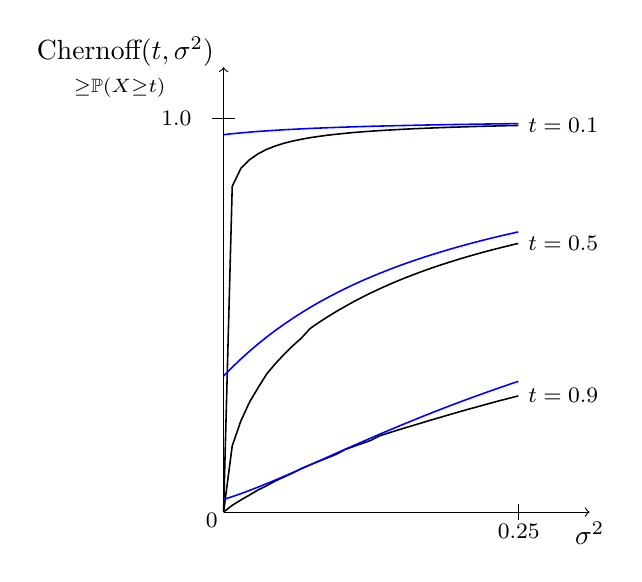
\begin{tikzpicture}[xscale=15, yscale=5]%[xscale=15, yscale=7.5]
\draw[->] (0,0) -- (0.31,0) node[anchor=north] {$\sigma^2$};
\draw[->] (0,0) -- (0,1.13) node[anchor=east, align=left] {$\text{Chernoff}(t,\sigma^2)$\\ $~~~~\scriptstyle\ge\pr(X\ge t)$};
\foreach \t in {0.1,0.5,0.9}{
	\draw[domain=0:0.25, color=black, line width=0.20mm, samples=35] 
		plot (\x,{((\x/(\x+\t))^(\x+\t)*(1.0/(1-\t))^(1-\t))^(1.0/(\x+1))}) node [right] {\footnotesize $t=\t$};
	\draw[domain=0:0.25, color=blue, line width=0.20mm, samples=35] 
		plot (\x,{e^(-\t*\t/(4*(1.0/17+\x/2)))}) node [right] {};
}

\draw (0.25,-0.02) -- (0.25,0.02);
\draw (-0.01,1) -- (0.01,1);
\draw	(0.25,-0.05) node{{\footnotesize $0.25$}}
		(-0.01,-0.02) node{{\footnotesize $0$}}
		(-0.04,1) node{{\footnotesize $1.0$}};
\end{tikzpicture}}
\end{figure} 


\begin{figure}
\floatbox[{\capbeside\thisfloatsetup{capbesideposition={right,center},capbesidewidth=6.4cm}}]{figure}[\FBwidth]
{\caption{Chernoff upper bounds derived directly from the moment generating functions of equations Equation~\eqref{eq:part1} and~\eqref{eq:part3} (in black and blue, resp.) with $D=1$; Plotted for various $t$ against the variance $\sigma^2$.
Note that Equation~\eqref{eq:part3} generally captures the shape and magnitude of the more accurate equation, except in the region of small $\sigma^2$ where the bound is overly weakened.}
\label{fig:graph2}}
{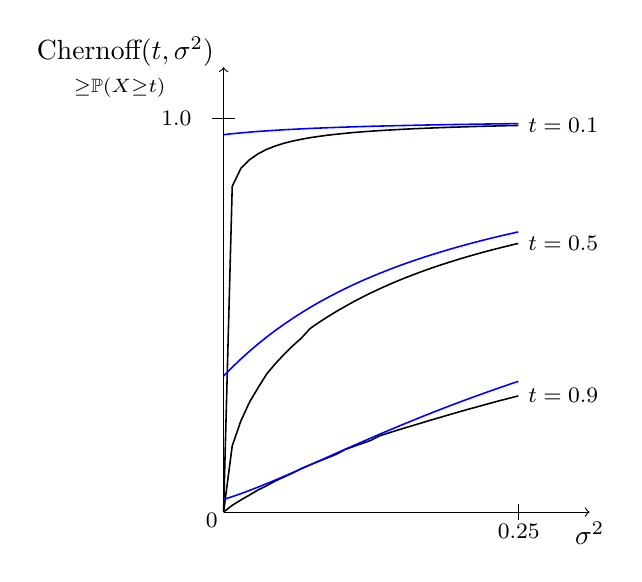
\begin{tikzpicture}[xscale=15, yscale=5]%[xscale=15, yscale=7.5]
\draw[->] (0,0) -- (0.31,0) node[anchor=north] {$\sigma^2$};
\draw[->] (0,0) -- (0,1.13) node[anchor=east, align=left] {$\text{Chernoff}(t,\sigma^2)$\\ $~~~~\scriptstyle\ge\pr(X\ge t)$};
\foreach \t in {0.1,0.5,0.9}{
	\draw[domain=0:0.25, color=black, line width=0.20mm, samples=35] 
		plot (\x,{((\x/(\x+\t))^(\x+\t)*(1.0/(1-\t))^(1-\t))^(1.0/(\x+1))}) node [right] {\footnotesize $t=\t$};
	\draw[domain=0:0.25, color=blue, line width=0.20mm, samples=35] 
		plot (\x,{e^(-\t*\t/(4*(1.0/17+\x/2)))}) node [right] {};
}

\draw (0.25,-0.02) -- (0.25,0.02);
\draw (-0.01,1) -- (0.01,1);
\draw	(0.25,-0.05) node{{\footnotesize $0.25$}}
		(-0.01,-0.02) node{{\footnotesize $0$}}
		(-0.04,1) node{{\footnotesize $1.0$}};
\end{tikzpicture}}
\end{figure}


One primary limitation of our method is that it rests on assumption of known data widths $D_i$ (and in the case of sampling-without-replacement, also on strata sizes $N_i$), which may not be exactly known in practice.
One way to overcome this may be to use our method with a reliable overestimate these parameters (by expert opinion or otherwise). This approximation or estimation may itself open consideration of other probability bounds and/or sampling methods, however we have not investigated this line of inquiry. 

In practice, it might also be advisable to run our method with an underestimate of the data widths, as the sampling process is fundamentally sensitive the the shape of the inequality and not necessarily its magnitude or accuracy as a bound.

% Our concentration inequality, Equation~\eqref{big_equation}, is derived by a combination of Chernoff bounds fused together with probability unions, so it is expected to give conservative confidence intervals on the error of the estimate in stratified random sampling, which may be useful outside of the context of sampling decisions.


\section{Multidimensional Extension}\label{sec:multi}

Our method of choosing samples can be extended to multidimensional data by a simple modification.
Specifically, instead of considering data that is single-valued, we consider data points that are vectors. 

Formally, for $n$ strata of finite data points which are all vectors of size $M$, let $n_i$ be the number of data points in the $i$th stratum.
Let the data in the $i$th stratum have a mean vector values $\mu_i$ (with $\mu_{i,j}$ for the $j$th component of the vector), which are value bounded within a finite width $D_{i,j}$, and have vector value variances $\sigma_{i,j}^2$.  
Given this, let $X_{i,1},X_{i,2},\dots,X_{i,n_i}$ (where $X_{i,k,j}$ is the $j$th component, of the $k$th vector from stratum $i$) be vector random variables corresponding to those data values randomly and sequentially drawn (with or without) replacement. 
Denote the average of the first $m_i$ of these random variables from the $i$th stratum by $\chi_{i,m_i}= \frac{1}{m_i}\sum_{k=1}^{m_i}X_{i,k}$ (with $\chi_{i,m_i,j}$ being the $j$th component of that vector average).
Let $\doublehat{\sigma}_{i,j}^2=\frac{i}{m_i-1}\sum_{k=1}^{m_i}(X_{i,k,j}-\chi_{i,m_i,j})^2$ be the unbiased sample variance of the first $m_i$ of these random variables in the $j$th component. 
As before, we assume weights $\tau_i$ for each stratum. \\
In this context we have the following theorem:

\begin{Theorem}[Vector SEBM bound]
In the context above, then with $\Omega_{m_i}^{n_i},\Psi_{m_i}^{n_i}$ per Lemma~\ref{martingale1}:
%\begin{equation}\label{big_equation2}\p\left(\begin{matrix*}[l]\sum_{j=1}^M\left(\sum_{i=1}^n\tau_i(\chi_{i,m_i,j}-\mu_{i,j})\right)^2 \ge \\ \quad\quad \log(6/p)\sum_{j=1}^M\begin{pmatrix*}[l]\sum_{i=1}^n\frac{4}{17}\Omega_{m_i}^{n_i}D_{i,j}^2\tau_i^2 \\ +\begin{pmatrix*}[l]\sqrt{\log(3/p)\left(\max_i\tau_i^2{\Psi_{m_i}^{n_i}}^2D_{i,j}^2\right)} \\ +\sqrt{\begin{matrix*}[l]2\sum_{i=1}^n\tau_i^2\Psi_{m_i}^{n_i}(m_i-1)\doublehat{\sigma}_{i,j}^2/m_i \\ + \log(6n/p)\sum_i\tau_i^2D_{i,j}^2\Omega_{m_i}^{n_i}\Psi_{m_i}^{n_i} \\ +\log(3/p)\left(\max_i\tau_i^2{\Psi_{m_i}^{n_i}}^2D_{i,j}^2\right)\end{matrix*}} \end{pmatrix*}^2\end{pmatrix*}\end{matrix*} \right)\le Mp \end{equation}

\begin{equation}\label{big_equation2}\pr\left(\begin{matrix*}[l]\sum_{j=1}^M\left(\sum_{i=1}^n\tau_i(\chi_{i,m_i,j}-\mu_{i,j})\right)^2 \ge \\ \quad\quad \log(6/p)\sum_{j=1}^M\left(\alpha_{m_i,j}^{n_i} +\left(\sqrt{\beta_{m_i,j}^{n_i}} +\sqrt{\gamma_{m_i,j}^{n_i}}\right)^2\right)\end{matrix*} \right)\le Mp \end{equation}

where:

\begin{align*}
\alpha_{j}=&\sum_{i=1}^n\frac{4}{17}\Omega_{m_i}^{n_i}D_{i,j}^2\tau_i^2 \\
\beta_{j}=&\log(3/p)\left(\max_i\tau_i^2{\Psi_{m_i}^{n_i}}^2D_{i,j}^2\right) \\
\gamma_{j}=&2\sum_{i=1}^n\tau_i^2\Psi_{m_i}^{n_i}(m_i-1)\doublehat{\sigma}_{i,j}^2/m_i
+ \log(6n/p)\sum_i\tau_i^2D_{i,j}^2\Omega_{m_i}^{n_i}\Psi_{m_i}^{n_i}  \\
&\quad\quad\quad\quad\quad\quad\quad\quad\quad\quad\quad~~+\log(3/p)\left(\max_i\tau_i^2{\Psi_{m_i}^{n_i}}^2D_{i,j}^2\right)
\end{align*}

%$$
%\alpha_{m_i,j}^{n_i}
%=\sum_{i=1}^n\frac{4}{17}\Omega_{m_i}^{n_i}D_{i,j}^2\tau_i^2 
%$$
%$$
%\beta_{m_i,j}^{n_i}
%=\log(3/p)\left(\max_i\tau_i^2{\Psi_{m_i}^{n_i}}^2D_{i,j}^2\right) 
%$$
%and
%\begin{align*}
%\gamma_{m_i,j}^{n_i}
%= 2\sum_{i=1}^n\tau_i^2\Psi_{m_i}^{n_i}(m_i-1)\doublehat{\sigma}_{i,j}^2/m_i
%&+ \log(6n/p)\sum_i\tau_i^2D_{i,j}^2\Omega_{m_i}^{n_i}\Psi_{m_i}^{n_i}  \\
%&+\log(3/p)\left(\max_i\tau_i^2{\Psi_{m_i}^{n_i}}^2D_{i,j}^2\right)
%\end{align*}

\end{Theorem}
\begin{proof}
Squaring \eqref{big_equation} and applying it specifically to the $j$th component of all the vectors gives:
\begin{equation*}
\pr\left(\frac{\left(\sum_{i=1}^n\tau_i(\chi_{i,m_i}-\mu_i)\right)^2}{\log(6/p)} 
\ge \alpha_{j} 
+ \left(\sqrt{\beta_{j}} 
+ \sqrt{\gamma_{j}}\right)^2  \right)
\le p 
\end{equation*}
%$$ \p\left(\frac{\left(\sum_{i=1}^n\tau_i(\chi_{i,m_i,j}-\mu_{i,j})\right)^2}{\log(6/p)}\ge \begin{matrix*}[l]\sum_{i=1}^n\frac{4}{17}\Omega_{m_i}^{n_i}D_{i,j}^2\tau_i^2 \\ +\begin{pmatrix*}[l]\sqrt{\log(3/p)\left(\max_i\tau_i^2{\Psi_{m_i}^{n_i}}^2D_{i,j}^2\right)} \\ +\sqrt{\begin{matrix*}[l]2\sum_{i=1}^n\tau_i^2\Psi_{m_i}^{n_i}(m_i-1)\doublehat{\sigma}_{i,j}^2/m_i \\ + \log(6n/p)\sum_i\tau_i^2D_{i,j}^2\Omega_{m_i}^{n_i}\Psi_{m_i}^{n_i} \\ +\log(3/p)\left(\max_i\tau_i^2{\Psi_{m_i}^{n_i}}^2D_{i,j}^2\right)\end{matrix*}} \end{pmatrix*}^2\end{matrix*} \right)\le p $$
Taking a series of union bounds (Lemma~\ref{prob_union}) over $j$ gives result.
\end{proof}

The left hand side of the inequality in \eqref{big_equation2} is the square Euclidean distance between our weighted stratified sample vector estimate $\sum_{i=1}^n\tau_i\chi_{i,m_i}$ and the true mean stratified vector $\sum_{i=1}^n\tau_i\mu_{i}$.
In this context, an example sampling process might consist of sampling to maximally minimize the right hand side of the inequality (similar to our SEBM process, described in Section~\ref{sec:SEBMalgorithm}).
This formulation can be applied to more involved computational tasks that involve sampling data with multiple features or auxiliary variables.


\section{Conclusions and Future Work}\label{sec:future}

%We begin this section with a discussion of the relationship of our bound to existing concentration inequalities, 
%and some opportunities for future improvements. 
The derivation of our inequality extends from consideration of Chernoff bounds and probability unions in a similar vein to other EBB derivations \citep{Maurer50empiricalbernstein,bardenet2015}.
%, however we do not argue that our particular concentration inequality is ideal.
However, the bounds on the moment generating functions that we developed in Section~\ref{sec:components} use loosening approximations, and hence stronger and/or more representative bounds could be developed at the cost of greater mathematical complexity.
Alternatively, an approach utilizing entropic \citep{Boucheron_concentrationinequalities} or Efron-Stein inequalities \citep{efron1981} could result in different and potentially tighter results.

% Additionally, although our method works generally, there may be better or more appropriate sampling methods in the event that there is more information known about the underlying distributions.
% It is sometimes possible to derive ideal concentration inequalities in restricted circumstances, and more broadly there exist some computational methods to numerically derive ideal bounds \citep{OUQ1,doi:10.1137/13094712X}.
% Using these techniques it may be possible to derive ideal numerical bounds, particularly for bounds considering very small numbers of samples.


We now consider prospective applications of our method. 
First, the approach derived in this paper was motivated by the problem of approximating the Shapley value of cooperative games defined over complicated optimization problems (i.e. with characteristic functions given by the solution to non-trivial optimization problems). 
Two examples of this are the problems of pricing (i) logistics, involving solutions to the travelling salesman problem \citep{AzizEtal2016}, and 
(ii) electricity networks, which requires solving optimzation problems that incorporate the power flow equations \citep{DBLP:journals/tsg/OBrienGR15,archie_paper1,ACUNA2018161,burgess_abstract}.
Focusing on electricity networks in particular: 
these are complicated technical system used to transport electrical power from generators to loads, 
subject to the non-linear physical and operational constraints of the system's components.
With the emergence of new technologies, electricity is now generated, monitored and used on neighborhood distribution networks by devices that are increasingly responsive and interconnected to the network. 
Because of this, there are various emerging schemes of how a future distribution-network energy market platform might be designed.
Within this context, the Shapley value has been proposed as a fair mechanism for the allocation of resources and costs on such networks.
The Shapley value has been considered in different ways as a mechanism for pricing demand response \citep{DBLP:journals/tsg/OBrienGR15}, demand or load \citep{archie_paper1}, supply or generation \citep{ACUNA2018161}, and potentially all simultaneously \citep{burgess_abstract}.
Although computing the Shapley value exactly is impractical in these contexts 
sample-based approximations are a promising avenue for implementing Shapely value pricing schemes in real-world electricity systems.

Second, a potential use of our stratified sampling method is in improving the performance of \textit{stochastic gradient decent} (SGD) methods for training neural networks \citep{2016arXiv160904747R}.
Neural networks are trained by iteratively refining their parameters --- the weights and biases of the network --- against a cost function of the network's performance against training data.
One common method of training neural networks is gradient decent (GD).
In each iteration of GD, the derivative of how much a change in any parameter would influence the average performance of the network across the training data is calculated as a gradient vector.
Once this vector is calculated, each network parameter takes a small step in the direction of this gradient, to incrementally increase the performance of the network, 
and through many of these steps the network becomes trained.

However in many cases, the entire corpus of training data is not used in each iteration but only a fraction of the corpus is sampled (as a `batch' or `minibatch'), and the average gradient vector of improved performance across the samples of the batch is calculated as an approximation of the true gradient vector. 
This iterative process has been called SGD, where one of the hyperparameters is the size of the batches, see \cite{DBLP:journals/corr/KeskarMNST16,l.2018dont}.
In the context of supervised learning, each element of the training data is labelled with the desired output of the neural network for it, and these labels can serve to naturally stratify the training data; or the data can be stratified by other means too \citep{DBLP:journals/corr/ZhangKM17,DBLP:journals/corr/abs-1804-02772,2014arXiv1405.3080Z}.
In this setting, Equation~\ref{big_equation2} may be used to choose between samples of labelled training data, in order to sample batches that more-efficiently estimate of the performance gradient, and hence improve the efficiency of neural network training procedure.
This idea of `smart sampling' for neural network training is not particularly new, and our method is potentially compatible with other performance-enhancing techniques in the literature on neural networks \citep{10.1007/978-3-319-24486-0_21,article123123131}.

% Full exploration of the potential applications are beyond the scope of this document.
% However, at present, we are pleased to present our analytic concentration inequality (Equation \ref{big_equation}) as an immediately computable expression and practical method for choosing samples from strata.\footnote{
Sourcecode for all the experiments in this paper are available at:\\ \href{https://github.com/Markopolo141/Stratified\_Empirical\_Bernstein\_Sampling}{https://github.com/Markopolo141/Stratified\_Empirical\_Bernstein\_Sampling
}


\section*{Acknowledgements}
A great thanks to Sylvie Thi\'{e}baux and Paul Scott for academic advice, encouragement and support!

\section*{Disclosure statement}
No potential conflict of interest was reported by the authors.

\bibliographystyle{tfnlm}
\bibliography{bib}




\appendix




\section{Parabola Fitting}\label{appendix1}

\begin{Theorem}\label{thm:parabola}
For $b>0$ and $a<b$ and $z>0$, there exists an $\alpha,\beta,\gamma$ such that: $\alpha x^2+\beta x+\gamma\ge \exp(x)$ for all $a\le x\le b$, and where:
$$z\alpha+\gamma = \frac{ze^b + b^2e^{-z/b}}{z + b^2}$$.
\end{Theorem}
\begin{proof}
An example parabola $\alpha x^2+\beta x+\gamma$ which that satisfies these requirements tangentially touches the exponential curve at one point (at $x=f<b$) and intersects it at another (at $x=b$), as illustrated in Figure \ref{fig:graph1}.
Thus the parabola's intersection at $x=b$ and its tangential intersection at $x=f$ can be written in matrix algebra:
$$
\begin{bmatrix}
    \alpha \\
    \beta \\
	\gamma
\end{bmatrix}
=
\begin{bmatrix}
    b^2 & b & 1 \\
    f^2 & f & 1 \\
	2f  & 1 & 0
\end{bmatrix}^{-1}
\begin{bmatrix}
    \exp(b) \\
    \exp(f) \\
	\exp(f)
\end{bmatrix}$$
This gives our parabola parameters $\alpha,\beta,\gamma$, in terms of $f$ and $b$, hence:\\
\-\hspace{3mm}$z\alpha+\gamma = (((z+fb-b)(f-b-1)-b)e^f+(f^2+z)e^b)(b-f)^{-2}$\\
Minimizing with respect to $f$ occurs at $f=\frac{-z}{b}$ and gives the result.
\end{proof}

\vspace{2cm}

\begin{figure}[h]
\centering
\begin{tikzpicture}[scale=1.0]
\draw[->] (-3.5,0) -- (2,0) node[anchor=north] {$x$};
\draw[->] (0,0) -- (0,4) node[anchor=east] {};
\draw[smooth, domain=-3.5:2.0, color=black, line width=0.20mm] 
    plot (\x,{e^(\x)/2}) node [right] {\footnotesize $e^x$};
\draw[smooth, domain=-3.5:2.0, color=red, line width=0.20mm] 
    plot (\x,{(0.316137167001903*\x*\x + 1.39988395124422*\x + 1.67055451771745)/2}) node [right] {\footnotesize $\alpha x^2+\beta x+\gamma$};
\draw (1.5,-0.1) -- (1.5,{e^(1.5)/2});
\draw (-2,-0.1) -- (-2,{e^(-2)/2});
\draw (-2.5,-0.1) -- (-2.5,0);
\draw[black,fill] (1.5,{e^(1.5)/2}) circle (0.25mm);
\draw[black,fill] (-2,{e^(-2)/2}) circle (0.25mm);
\draw	(-2.5,-0.25) node{{\scriptsize $c$}}
		(-2,-0.25) node{{\scriptsize $f$}}
		(1.5,-0.25) node{{\scriptsize $d$}};
\end{tikzpicture}
\caption{A parabola parametarized by touching and intercepting points $f,b$ above an exponential curve for all $a\le x\le b$}
\label{fig:graph1}
\end{figure}

\begin{figure}[h]
\centering
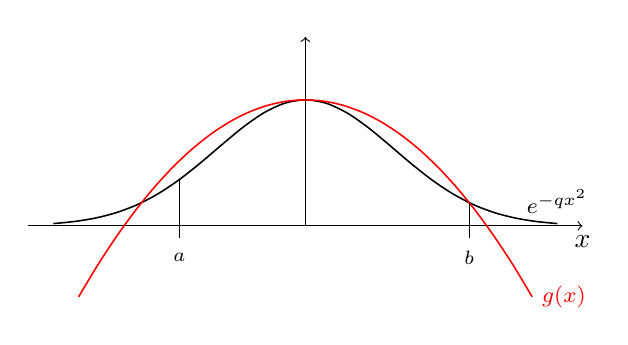
\begin{tikzpicture}[scale=1.6]
\draw[->] (-2.2,0) -- (2.2,0) node[anchor=north] {$x$};
\draw[->] (0,0) -- (0,1.5) node[anchor=east] {};
\draw[smooth, domain=-2.0:2.0, color=black, line width=0.20mm] 
    plot (\x,{e^(-(\x*\x))}) node [above] {\footnotesize $e^{-qx^2}$};
\draw[smooth, domain=-1.8:1.8, color=red, line width=0.20mm] 
    plot (\x,{-0.4825*\x*\x+1}) node [right] {\footnotesize $g(x)$};
\draw (1.3,-0.1) -- (1.3,{e^(-1.3*1.3)});
\draw (-1,-0.1) -- (-1,{e^(-1*1)});
\draw	(-1,-0.25) node{{\scriptsize $a$}}
		(1.3,-0.25) node{{\scriptsize $b$}};
\end{tikzpicture}
\caption{Parabola $g(x)=(\exp(-qd^2)-1)d^{-2}x^2+1$ over function $f(x)=\exp(-qx^2)$ for all $a\le x\le b$ where $d=\max(b,-a)$; in the case $a=-1,b=1.3,q=1$}\label{fig:graph111}
\end{figure}



\end{document}
